\chapter{Testy i wyniki}
\label{cha5}

W tym rozdziale zostały przedstawione wszystkie wykonane badania wraz z ich wynikami. W badaniach zostały uwzględnione wszystkie metody uczenia maszynowego przedstawione w rozdziale \ref{cha:ucz.masz} rozszerzając podejścia przytoczone w przeglądzie literatury (rozdział \ref{cha:stan.badan}). Badania te stanowią uzupełnienie i rozszerzenie prac z \cite{Reczek21}. 

\section{Opis podejścia}
\label{opis_podejścia}
%  (czym się różni od tego z rozdz. 2)
Badania te zostały podzielone na dwa duże etapy. Pierwszy z nich polegał na rozpoznawaniu pojedynczych struktur obecnych na zdjęciach mikrostruktur. Wiązało się to z wyznaczeniem konturów tych obiektów, następnie ich wycięcie i utworzenie z nich bazy danych, co wymagało “ręcznego” przyporządkowania obrazów do siedmiu klas. Następnie, za pomocą tego zestawu danych możliwe byłoby wyuczenie sieci neuronowej rozpoznającej te kształty. Eksperymenty rozpoczęto przetestowania momentów Hu oraz tekstur Haralicka w celu sklasyfikowania całych zdjęć mikrostruktur i stwierdzenia których kształtów jest najwięcej. Następnym krokiem było przetestowanie uogólnionej transformaty Hougha. Po zakończeniu tych testów rozpoczęto badania nad bardziej skomplikowanymi metodami, które można byłoby zastosować bardziej automatycznie. Szczegóły dotyczące wycinania, tworzenia bazy danych i rozpoznawania tych struktur zostały przedstawione w rozdziałach \ref{wycinanie.struktur} oraz \ref{klasyfikacja.struktur}, które to zostały w całości poświęcony temu etapowi.

Drugi etap polegał na ocenie jakości odlewów za pomocą technik wypracowanych w pierwszej fazie, wykorzystując klasyczne klasyfikatory, ale również posługując się sieciami neuronowymi. W pierwszej kolejności wykorzystano momenty Hu w celu wyłuskania z obrazów cech, za pomocą których można byłoby przeprowadzić klasyfikację. Analogicznie przetestowano tekstury Haralicka. Cechy te podawano na wejście klasycznych klasyfikatorów, które zostały przedstawione w rozdziale \ref{cha:Wykorzystane metody uczenia maszynowego}. Następnie przeprowadzono kompleksowe badania, w których wykorzystywano liczbę struktur konkretnych klas znajdujących się na zdjęciach mikrostruktur, a także klasyczne klasyfikatory. Wszystkie otrzymane wyniki porównano uwzględniając wiele aspektów, jak interpretowalność wyników, łatwość implementacji, prostotę algorytmu czy czas uczenia. Aby mieć ogląd całej sytuacji przetestowano również najskuteczniejsze obecnie architektury sieci neuronowych wykorzystywanych w celach klasyfikacji obrazów i również zostały one porównane wielopłaszczyznowo z pozostałymi wynikami.

% ############ Klasyfikacja struktur #############
\section{Klasyfikacja struktur}
\label{sec:klasyfikacja_struktur}

Jest to najszerszy obszar badań, ponieważ dzięki danym w postaci zliczonych struktur można sprawdzić, czy kształty tych struktur mają wpływ na właściwości mechaniczne odlewów, a jeśli tak, to w jakim stopniu. Jak dobrze wiadomo, sieci neuronowe, które otrzymują obrazy w postaci pikseli jako dane wejściowe i zwracają wynik w postaci „tak” lub „nie” odpowiadając na pytanie, czy wytrzymałość na rozciąganie danej mikrostruktury jest duża (lub mała) są modelami „czarnej skrzynki”, co oznacza, że trudno zweryfikować, dlaczego model podjął jedną decyzję nad drugą. Wykorzystując jednak dane w postaci liczby struktur i ich klas, można pokusić się o zbudowanie interpretowalnego modelu. W tym celu zostanie przetestowany szereg metod, z pomocą których będziemy w stanie wyodrębnić poszczególne obiekty na zdjęciach mikrostruktur, a następnie, za pomocą modelu sieci neuronowej będziemy mogli je rozpoznować. 

% ############ Klasyfikacja struktur ###################
\subsection{Uogólniona transformata Hougha}
\label{hough}

Jako pierwsze podejście zostały przetestowane momenty Hu oraz tekstury Haralicka, aczkolwiek zostały one również wykorzystane w celu oceny jakości odlewów. Zasada działania była podobna, aczkolwiek była ona bardziej rozbudowana w celu oceny jakości odlewów, stąd odsyłamy do rozdz. \ref{sec:hu_haralick}, gdzie zostały szczegółowo opisane. W tym rozdziale zajmiemy się uogólnioną transformatą Hougha (ang. \ita{generalised Hough transform}, \bo{GHT}), która została przebadana jako następna. Wykorzystano w tym celu otwartoźródłową bibliotekę \ita{general-hough}. 
\begin{figure}[h]
    \centering
    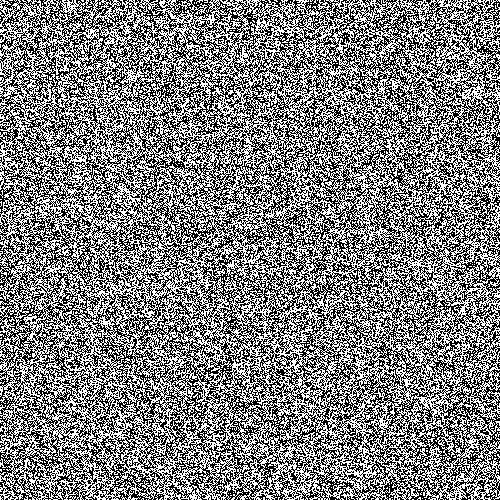
\includegraphics[width=0.5\textwidth]{rys.21.ght.duza.kulka.png}
    \caption{Wykrywanie kształtu przedstawionego na obrazie referencyjnym (ang. \ita{reference image}) na obrazie zapytania (ang. \ita{query image}). W prawym dolnym rogu na czerwono zaznaczono wykryte kształty. Żółty krzyżyk oznacza najtrafniejszy punkt. Obraz referencyjny w tym przypadku to czarne koło. Żródło: opracowanie własne przy wykorzystaniu biblioteki \ita{general-hough}}
    \label{fig:mesh21}
\end{figure}
Ta strategia jest bardziej skoncentrowana na pojedynczych strukturach i ich detekcji. Początkowe zmagania pokazały, że znajdowanie pojedynczych struktur danej klasy z pomocą tej metody jest możliwe, aczkolwiek nie wszystkie kształty, a niekiedy zdarzają się nawet większe pomyłki, co przedstawiono na poniższych obrazkach (rys. \ref{fig:mesh21}, \ref{fig:mesh22} i \ref{fig:mesh23}). Chociaż uważa się, że GHT ma zalety, takie jak:
\begin{itemize}
	\item odporność na częściowe lub nieznaczne zniekształcenie formy
	\item odporność na obecnoć innych struktur na obrazie,
	\item odporność na szum,
	\item możliwość znajdowania wielu wystąpień danego kształtu na obrazie wejściowym.
\end{itemize}
Pomimo tego, że metoda ta została stworzona właśnie do rozpoznawania form zdefiniowanych matematycznie (takie występują na naszych obrazach), jego działanie nie spełniło naszych oczekiwań.
\begin{figure}[h]
    \centering
    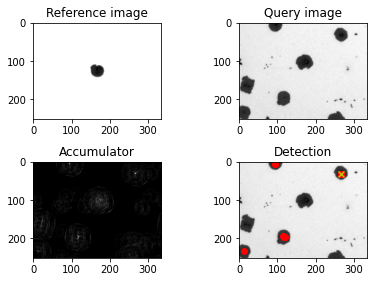
\includegraphics[width=0.6\textwidth]{rys.22.ght.mala.kulka.png}
    \caption{Działanie metody GHT na tym samym obrazie zapytania, lecz jako obraz referencyjny została użyta rzeczywista struktura znajdująca się na jednym ze zdjęć. Dodatkowo skala tej struktury jest taka sama, jak skala struktur na obrazie zapytania. Żródło: opracowanie własne przy wykorzystaniu biblioteki \ita{general-hough}}
    \label{fig:mesh22}
\end{figure}
Jak widać na rysunku \ref{fig:mesh21}, w oczy rzucają się dwa problemy. Po pierwsze, nie wykryto wszystkich kształtów. Po drugie, czerwone kropki oznaczające wykryty kształt niekiedy znajdują się na szarym tle, zamiast na czarnym kształcie. Ale to nie jedyne problemy. Zdarza się również, iż dana struktura jest oznaczona wielokrotnie. Dlatego zdecydowano się poeksperymentować z obrazami referencyjnymi, co potencjalnie może poprawić wyniki. Na kolejnym rysunku \ref{fig:mesh22} możemy zauważyć, że obraz zapytania jest wciąż ten sam, natomiast zmienił się obraz referencyjny. Tym razem jest to rzeczywista struktura, a więc nie jest ani idealnia czarna, ani idealnie okragła. Dodatkowo jej skala jest taka sama, jak skala struktur na obrazie zapytania. Możemy również zaobserwować na obrazie z wykrytymi kształtami (ang. \ita{detection}), iż tym razem czerwone kropki są rozmieszczone o wiele bardziej precyzyjne. 
\begin{figure}[h]
    \centering
    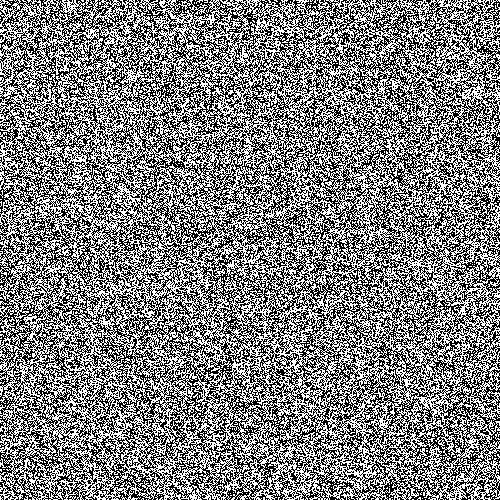
\includegraphics[width=0.6\textwidth]{rys.23.ght.mala.kulka.bez.szarosci.png}
    \caption{Kolejny test z tym samym obrazem zapytania, a także z tym samym obrazem referencyjnym, co na rys. \ref{fig:mesh22}. Widzimy, że metoda zadziałała jeszcze lepiej, gdyż wykryła poprawnie jeszcze jedną strukturę. Żródło: opracowanie własne przy wykorzystaniu biblioteki \ita{general-hough}}
    \label{fig:mesh23}
\end{figure}
Jednakże wciąż metoda ta nie jest na wystarczająco dokładna. W kolejnych testach usunięto dodatkowo szare tło z obrazów zapytania, przez co szare struktury znalazły się po tych przekształceniach na białym tle. Przykładowe wyniki zostały zaprezentowane na obrazie \ref{fig:mesh23}. Możemy zauważyć, że ten zabieg przyniósł oczekiwane efekty, a mianowicie wykryto poprawnie o jeden kształt więcej, niż przed tym zabiegiem.
Mimo wszystko takie podejście jest mało praktyczne, gdyż dla różnych obrazów należałoby dobierać obrazki referencyjne zgodnie ze skalą struktur na obrazach. Dodatkowo, pomimo tego, iż jest zaledwie sześć klas tych struktur, potrzebowalibymy znacznie więcej przykładów, aby pokryć przypadki, w których struktura jest zniekształcona, bądź nakłada się z inną strukturą. A więc wiemy już, że ta metoda nie może zostać wykorzystana w dalszych badaniach, a zatem należy wrócić do poszukiwań tej odpowiedniej metody.

\subsection{Detekcja krawędzi filtrem Canny'ego}
\label{canny}

Kolejne techniki były bardziej skoncentrowane na wycinaniu poszczególnych struktur, a następnie kategoryzowaniu każdej z nich niezależnie w kolejnych fazach. W tym celu wykorzystano pakiet \ita{opencv-python} (nazywana dalej \ita{cv}). Jednak w pierwszym kroku opracowano algorytm do przeprowadzania prostego zliczania struktur bez rozróżniania klasy kształtu. Krawędzie struktur wykrywano metodą Canny'ego \cite{Canny86}. Dodatkowo przetestowano różne techniki rozmywania obrazu (ang. \ita{blur}), czy inaczej – wygładzania, m.in. uśrednianie (w pythonie \ita{cv.blur}), rozmycie gaussowskie (ang. \ita{Gaussian blur}, w pythonie \ita{cv.GaussianBlur}), rozmycie środkowe (ang. \ita{median blurring}, w pythonie \ita{cv.medianBlur}) i filtrowanie dwustronne (ang. \ita{bilateral filtering}, w pythonie \ita{cv.bilateralFilter}). 
W zależności od rozmiaru zastosowanego jądra (ang. \ita{kernel}) otrzymujemy różne efekty przy rozmyciu. Rysunek \ref{fig:mesh24} przedstawia trzy zdjęcia, z których jeden jest oryginalny (pierwszy od prawej), a dwa pozostałe to efekt zastosowania wykrywania krawędzi. W pierwszym od lewej zastosowano antyaliasing (rozmiar jądra 5x5), podczas gdy w środkowym obrazie nie.
\begin{figure}[h]
	\centering
	\begin{subfigure}{0.29\textwidth}
	    \centering
	    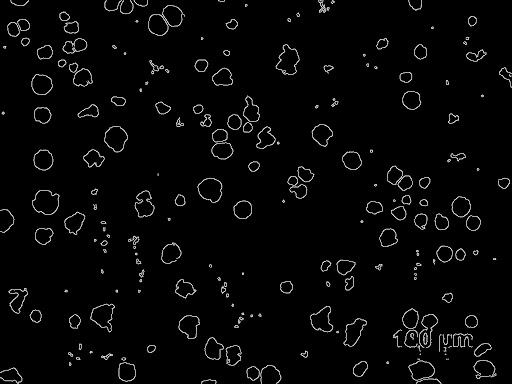
\includegraphics[width=1\textwidth]{rys.25a.canny.antialiasing.jpg} % pominalem obrazek 24, moze dodam kiedys
	    \subcaption{\label{subfigure_a}Wykrywanie krawędzi z wykorzystaniem wygładzania}
	\end{subfigure}
	\begin{subfigure}{0.29\textwidth}
	    \centering
	    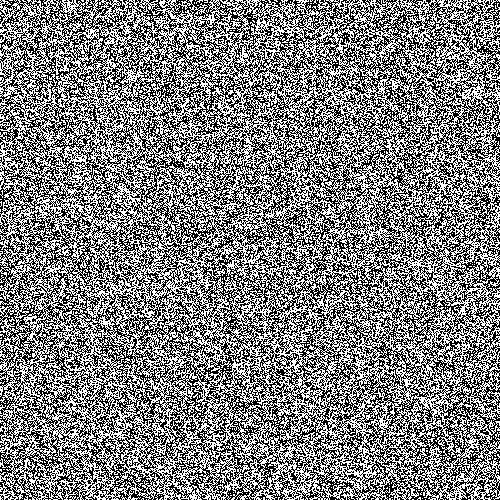
\includegraphics[width=1\textwidth]{rys.25b.canny.jpg}
	    \subcaption{\label{subfigure_b}Wykrywanie krawędzi na oryginalnym obrazku}
	\end{subfigure}
	\begin{subfigure}{0.29\textwidth}
	    \centering
	    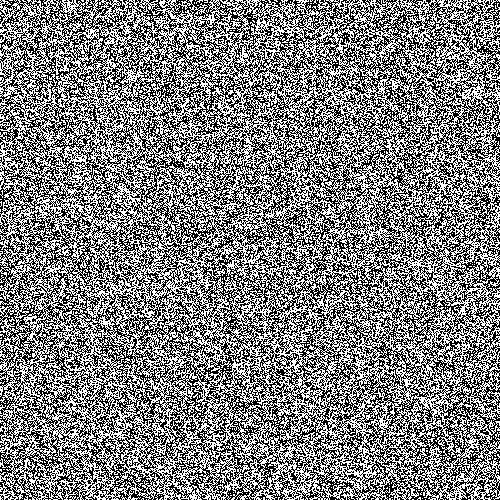
\includegraphics[width=1\textwidth]{rys.25c.canny.original.jpg}
	    \subcaption{\label{subfigure_c}Oryginalne zdjęcie mikrostruktury}
	\end{subfigure}
	\caption{\label{fig:mesh24}Wykrywanie krawędzi z wykorzystaniem filtra Canny'ego. Źródło: opracowanie własne}
\end{figure}
Wykryte struktury zostały następnie zliczone. Są to wszystie kontury widoczne na dwóch pierwszych obrazkach na rys. \ref{fig:mesh24}. Rysunek \ref{fig:mesh25} przedstawia przykład obrazu, dla którego algorytm wyliczył dziesięć takich struktur (czy też konturów).
\begin{figure}[h]
    \centering
    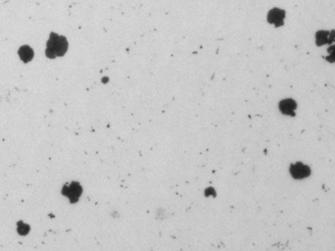
\includegraphics[width=0.35\textwidth]{rys.26.sample.image.strusctures.counting.png}
    \caption{Przykładowe zdjęcie mikrostruktury, dla którego wykryto 10 kształtów}
    \label{fig:mesh25}
\end{figure}
Zliczanie konturów przeprowadzono w taki sposób, iż dla każdego obiektu obliczono pole powierzchni i obwód. W ten sposób można odrzucić kontury o małej powierzchni lub małym obwodzie. Wszystkie drobne, nieistotne kształty są eliminowane za pomocą tego podejścia. Podczas prób przebadano również takie metody, jak progowanie (ang. \ita{threshold}), dylatacja (ang. \ita{dilation}), erozja (ang. \ita{erosion}) i morfologia (ang. \ita{morphology}), jednakże najlepsze wyniki osiągnięto podczas zliczania struktur na oryginalnym zdjęciu.

\subsection{Wycinanie pojedynczych struktur z obrazków}
\label{wycinanie.struktur}

Następnie, posiadając program (przygotowany samodzielnie), z pomocą którego jesteśmy w stanie wyznaczać kontury struktur, możemy spróbować je wycinać. Przyjęto strategię wycinania pojedynczych obiektów, a następnie nakładania ich na białe tło. Struktury były umieszczane w środku obrazu o białym tle o wymiarach 335 x 251 (szer. x wys.). Przykładowa wycięta struktura znajduje się na rys. \ref{fig:mesh26}.
\begin{figure}[h]
    \centering
    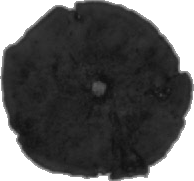
\includegraphics[width=0.25\textwidth]{rys.27.przykladowa.wycieta.struktura.png}
    \caption{Przykładowe zdjęcie wyciętej struktury (obraz przybliżony). Pozostałe kształty są wycinane analogicznie}
    \label{fig:mesh26}
\end{figure}
Poniższe obrazki (rys. \ref{fig:mesh26} i \ref{fig:mesh27}) przedstawiają działanie tego procesu. Tym samym kolorem zostały zaznaczone kształty, które zostały potraktowane jako jeden obiekt. Natomiast na rys. \ref{fig:mesh28} możemy zobaczyć przykładowe struktury, które zostały wycięte ze zdjęcia przedstawionego na rys. \ref{fig:mesh26}. 
\begin{figure}[h]
	\centering
	\begin{subfigure}{0.29\textwidth}
	    \centering
	    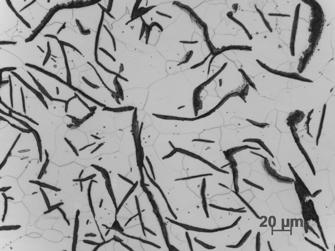
\includegraphics[width=1\textwidth]{rys.28a.wycinanie.struktur.png}
	    \subcaption{\label{subfigure_a}Zdjęcie mikrostruktury}
	\end{subfigure}
	\begin{subfigure}{0.29\textwidth}
	    \centering
	    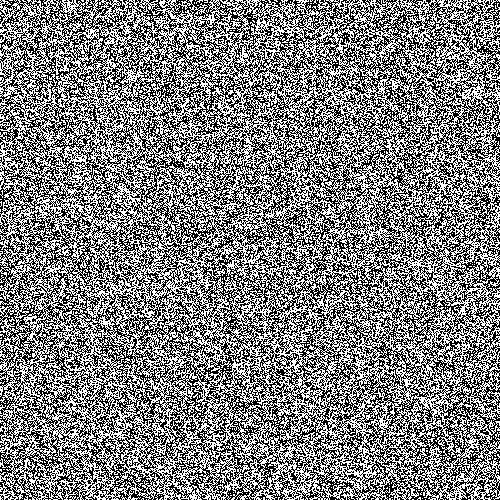
\includegraphics[width=1\textwidth]{rys.28b.wycinanie.struktur.png}
	    \subcaption{\label{subfigure_b}Wykryte struktury}
	\end{subfigure}
	\caption{\label{fig:mesh26}Działanie filtra Canny'ego. Każda wykryta struktura jest zaznaczona innym kolorem. Źródło: opracowanie własne}
\end{figure}
Struktury na obrazku oznaczone tym samym kolorem (a zatem uznane jako pojedynczy obiekt) są wycinane i umieszczane na białym tle. Zostaną one wykorzystane do trenowania modeli kategoryzacji w kolejnych fazach. Z drugiej strony, jak widać na powyższym obrazie, wadą tej techniki jest to, że struktury są czasami ze sobą połączone, a następnie traktowane przez algorytm jako jedna całość. Dzieje się tak najczęściej w przypadku klas I i II (rys. \ref{fig:mesh14}), które są rozciągnięte na zdjęciach i często się stykają ze sobą. 
\begin{figure}[h]
	\centering
	\begin{subfigure}{0.29\textwidth}
	    \centering
	    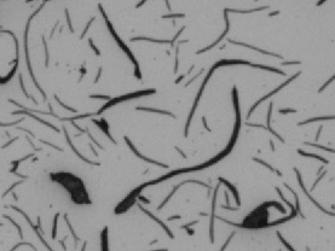
\includegraphics[width=1\textwidth]{rys.29a.wycinanie.struktur.png}
	    \subcaption{\label{subfigure_a}Zdjęcie mikrostruktury}
	\end{subfigure}
	\begin{subfigure}{0.29\textwidth}
	    \centering
	    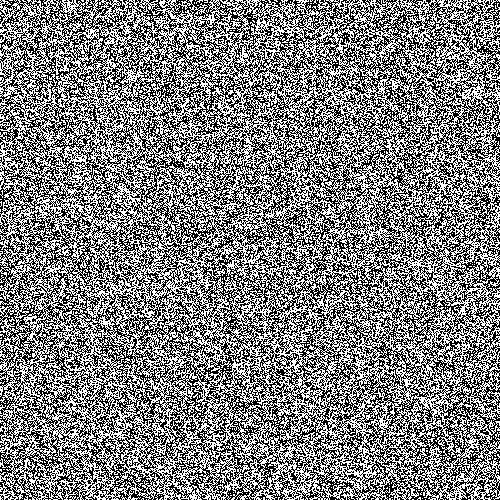
\includegraphics[width=1\textwidth]{rys.29b.wycinanie.struktur.png}
	    \subcaption{\label{subfigure_b}Wykryte struktury}
	\end{subfigure}
	\caption{\label{fig:mesh27}Kolejny przykład działania filtra Canny'ego. Każda wykryta struktura jest zaznaczona innym kolorem. Źródło: opracowanie własne}
\end{figure}
Próbowano tego uniknąć za pomocą takich algorytmów, jak erozji i progowania, ale te podejścia nie przyniosły zamierzonych rezultatów. Poniżej inny przykład działania tego samego algorytmu.
Algorytm na rys. \ref{fig:mesh26} zadziałał nieco lepiej niż na rys. \ref{fig:mesh26}. Jak widać, większość elementów została wycięta osobno. Tylko połączone kształty zostały wycięte jako jedna całość. Niestety nie ma na to uniwersalnego rozwiązania, ponieważ gdy ten problem zostanie rozwiązany, pojawia się nowy, jak np. brak wycinania mniej widocznych struktur lub wykrywanie wyblakłych struktur, które powinny zostać pominięte.
\begin{figure}[h]
	\centering
	\begin{subfigure}{0.29\textwidth}
	    \centering
	    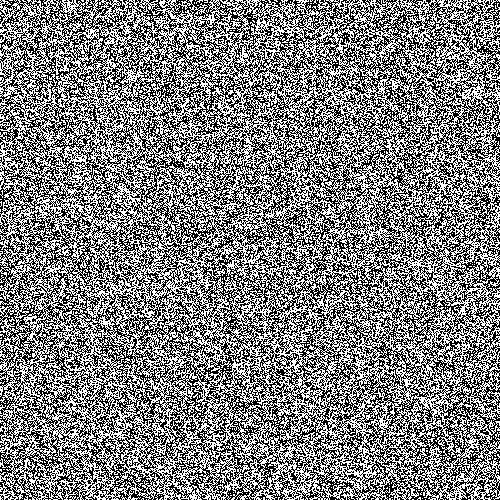
\includegraphics[width=1\textwidth]{rys.30a.wyciete.obiekty.png}
	\end{subfigure}
	\begin{subfigure}{0.29\textwidth}
	    \centering
	    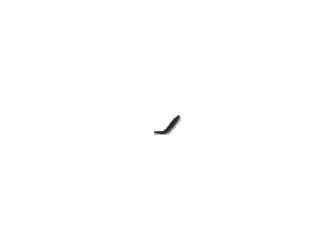
\includegraphics[width=1\textwidth]{rys.30b.wyciete.obiekty.png}
	\end{subfigure}
	\begin{subfigure}{0.29\textwidth}
	    \centering
	    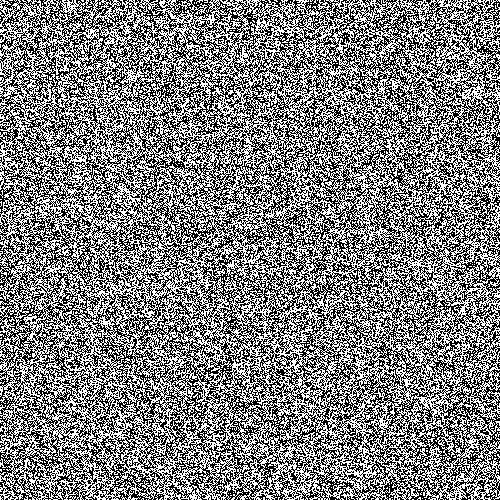
\includegraphics[width=1\textwidth]{rys.30c.wyciete.obiekty.png}
	\end{subfigure}
	\begin{subfigure}{0.29\textwidth}
	    \centering
	    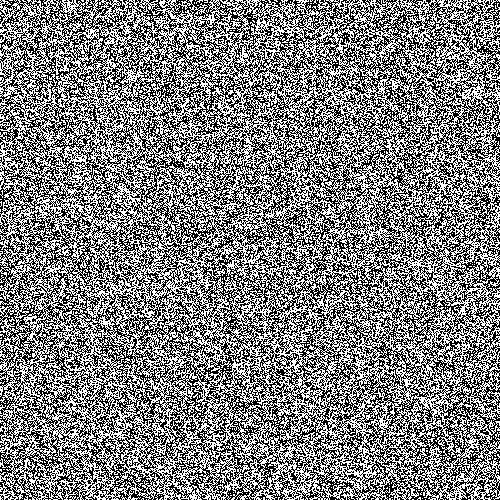
\includegraphics[width=1\textwidth]{rys.30d.wyciete.obiekty.png}
	\end{subfigure}
	\begin{subfigure}{0.29\textwidth}
	    \centering
	    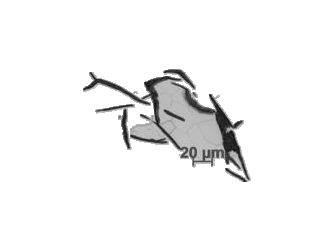
\includegraphics[width=1\textwidth]{rys.30e.wyciete.obiekty.png}
	\end{subfigure}
	\begin{subfigure}{0.29\textwidth}
	    \centering
	    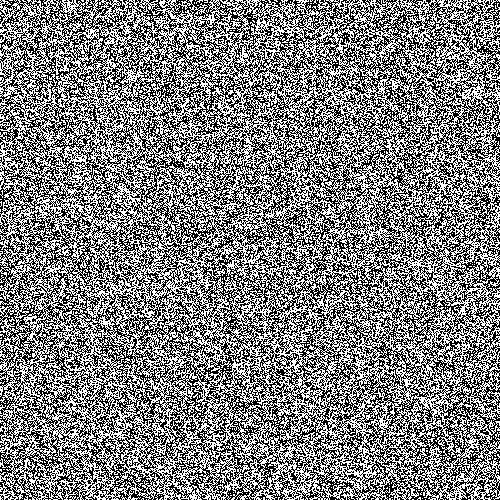
\includegraphics[width=1\textwidth]{rys.30f.wyciete.obiekty.png}
	\end{subfigure}
	\caption{\label{fig:mesh28}Przykładowe wycięte struktury z rys. \ref{fig:mesh26}. Źródło: opracowanie własne}
\end{figure}
Wycięte w ten sposób obiekty (rys. \ref{fig:mesh28}) są wprowadzane na wejście sieci neuronowej (rozdział \ref{klasyfikacja.struktur}), która zostanie wytrenowana do kategoryzowania tych struktur. W naszym zbiorze mamy siedem różnych klas. Sześć z nich (rys. \ref{fig:mesh14}) to kształty wyróżnione w normie \cite{norma}, natomiast autor dodał klasę siódmą, aby odróżnić te struktury od obiektów, które zostałe źle wycięte lub zawierających skalę, którą można znaleźć na wszystkich zdjęciach mikrostruktur. Wszystkie wycięte elementy były przechowywane lokalnie i arbitralnie przypisywane do klas podczas tworzenia zbioru danych. Liczność tych klas jest następująca:
\begin{itemize}[label=\textbullet]
	\item klasa 0 – 14 przykładów (dodana przez autora),
	\item klasa I – 278 przykładów,
	\item klasa II – 122 przykładów,
	\item klasa III – 292 przykładów,
	\item klasa IV – 76 przykładów,
	\item klasa V – 289 przykładów,
	\item klasa VI – 501 przykładów.
\end{itemize}
W następnym podrozdziale (tj. \ref{klasyfikacja.struktur}) zostały zaprezentowane badania związane z klasyfikacją wyciętych struktur.

\subsection{Rozpoznawanie wyciętych struktur}
\label{klasyfikacja.struktur}

Na tym etapie badań posiadamy już własnoręcznie przygotowane dane dotyczące pojedynczych struktur obecnych na zdjęciach mikrostruktur (rys. \ref{fig:mesh14}). Ponownie, można by zacząć eksperymenty od takich najprostszych metod, jak momenty Hu, momenty Zernike i tekstury Haralicka wraz z klasycznymi klasyfikatorymi, aczkolwiek takie podejście zostało już sprawdzone w pracy \cite{Reczek21} i pokazano, iż w przypadku takich zestawów algorytmów oraz dostępnych danych, wyniki są porównywalne do tych, które otrzymujemy w przypadku wykorzystania klasyfikatorów klasycznych z weśjciem w postaci pikseli. Dlatego tutaj przejdziemy od razu do bardziej zaawansowanych metod. W tym celu zdecydowano się wykorzystać sieci neuronowe (patrz \ref{cha:Siecineuronowe}). W szczególności zastosowano uczenie transferowe (patrz \ref{cha:cha3.5}) wykorzystując dobrze znaną sieć VGG19. 
\begin{figure}[h]
    \centering
    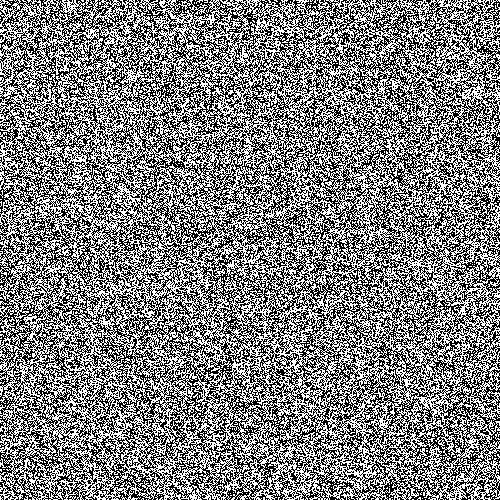
\includegraphics[width=0.75\textwidth]{rys.31.confusion.matrix.better.quality.png}  %rys.31.confusion.matrix.png}
    \caption{Tablica pomyłek dla klasyfikacji struktur znajdujących się na zdjęciach mikrostruktur dla danych testowych. Żródło: opracowanie własne (z użyciem biblioteki \ita{seaborn})}
    \label{fig:mesh29}
\end{figure}
Implementacja tej architektury została uzyskana z biblioteki \ita{Keras}. Podczas szkolenia sieć ta była wyłączona z treningu. Dodatkowo jej końcówka nie została zawarta, natomiast dodano kilka dodatkowych warstw, które pozwoliły nam na douczenie sieci pod nasze dane. Zastosowano optymizator \ita{Adam}, wielkość paczki uczącej (ang. \ita{batch size}) wyniosła jeden, natomiast liczba epok wyniosła 100 (rys. \ref{fig:mesh30}).  Taka sieć średnio osiąga wydajność około 82\% dla danych testowych (w przypadku danych treningowych dokładność waha się od 86\% do 95\% wydajności, w zależności od konfiguracji), wartość metryki F1 wynosi 0.79, natomiast wartość straty logistycznej (ang. \ita{logistic loss}) wyniosła 0.66. Są to lepsze wyniki niż w przytoczonej wczeniej pracy \cite{Reczek21} ze względu na to, że pracujemy na poprawionych danych, co zostało szczegółowo opisane w przytoczonej pracy. Rysunek \ref{fig:mesh29} przedstawia tablicę pomyłek, znormalizowaną względem wierszy (tj. rzeczywistych wartości). 
Po przeliczeniu na błąd względny otrzymujemy błędy na poziomie 10\%, 52\%, 26\%, 50\%, 49\% oraz 1\% odpowiednio dla klas od I do VI (brak klasy „0” w danych testowych ze względu na ich niską liczność). Błędy wynikają jednak głównie z podobieństwa tych form w ramach „sąsiadujących” klas, takich jak klasy V i VI (na rysunku są to klasy 4 i 5), gdzie prawie połowa kształtów z klasy V jest sklasyfikowana jako klasa VI. Podobieństwo klas można dostrzec również na rys. \ref{fig:mesh14}, aczkolwiek jest to bardziej widoczne w przypadku rzeczywistych danych, ponieważ większość tych kształtów zawiera cechy wielu klas (trudno im przypisać jedną konkretną cechę). Co więcej, baza danych została zbudowana arbitralnie przez osobę, kto nie jest ekspertem w dziedzinie metalurgii. Rozbieżności w dokładności predykcji między klasami są najprawdopodobniej związane z brakiem zbalansowania w ilości danych dostępnych dla każdej klasy.
\begin{figure}[h]
    \centering
    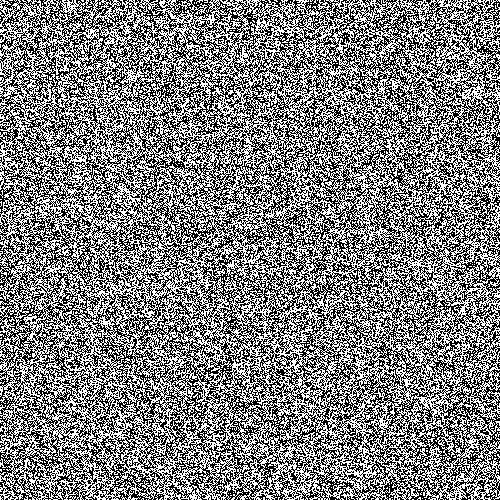
\includegraphics[width=0.55\textwidth]{rys.32.vgg19.history.lepsza.jakosc.png}
    \caption{Historia dokładności modelu sieci neuronowej w trakcie uczenia się. Są to rezultaty dla danych treningowych, gdzie najlepsze wyniki sięgają 87\%. Żródło: opracowanie własne (z wykorzystaniem biblioteki \ita{seaborn})}
    \label{fig:mesh30}
\end{figure}
Z drugiej strony wyniki wydają się być znacznie lepsze przy wykorzystaniu danych treningowych do ewaluacji. Po przeliczeniu błędów względnych otrzymujemy następujące wyniki: 36\% (klasa “0”), 0.4\%, 20\%, 7\%, 19\%, 38\% oraz 3\%. Możemy zaobserwować, że dane uczące mają znacznie mniej błędów względnych, co wskazuje, że wyniki można jeszcze poprawić. Dobrym kierunkiem może być zbalansowanie danych, gdyż, jak można zauważyć, najlepsze wyniki otrzymujemy dla klas, których liczba instancji była największa w zbiorze (z wyjątkiem klasy V, aczkolwiek przykłady tej klasy są łudząco podobne do przykładów z klasy VI). Przyjęto więc strategię, aby rozszerzyć dane z tych klas, które jednocześnie mają najniższą skuteczność i najmniej przykładów. Stąd zostaną rozszerzone klasy: „0", II, IV oraz V. Ponownie zostanie zastosowana (podobnie jak w \ref{sec:hu_haralick}) metoda odbicia, która nie zmienia rozmiarów zdjęcia. Również tym razem zostanie zastosowana metoda odbicia horyzontalnego. Oprócz tego przetestowano jeszcze kilka innych podejść, jak nałożenie szumu na rozszerzone przykłady danych, a także usunięcie szarości z obrazów. Wyniki zostały przedstawione w tab. \ref{structures.classification.different.approaches}. 
\begin{table}[h]
	\centering
	\begin{threeparttable}
		\caption{Podsumowanie różnych podejść co do klasyfikacji kształtów. Źródło: opracowanie własne}
		\label{structures.classification.different.approaches}
		\begin{tabularx}{1\textwidth}{ |X|X|X|X| }
		  \hline
		   \textbf{Augmentacja} & \textbf{Zaszumienie} & \textbf{Usuwanie szarości} & \textbf{Dokładność}\\

		  \hline
		  Nie & Nie & Nie & \bo{82.2\%}\\

		  \hline
		  Tak & Nie & Nie & 78\%\\

		  \hline
		  Tak & Tak & Nie & 79.7\%\\

		  \hline
		  Tak & Tak & Tak & 77.1\%\\
  		  
		  \hline
		  Tak (dod. klasę III) & Tak & Tak & 74.9\%\\
  		  
		  \hline
		\end{tabularx}
	\end{threeparttable}
\end{table}
A więc, jak możemy zauważyć, manipulacja danymi nie wpłynęła pozytywnie na wynik klasyfikacji. W związku z tym dalsze badania zostaną przeprowadzone na architekturze, dla której osiągnięto najlepsze wyniki. Biorąc pod uwagę niezbalansowanie klas oraz to, iż te dane były przygotowywane ręcznie przez autora tej pracy (który nie jest specjalistą w dziedzinie metalurgii), w celu poprawy wyników tej klasyfikacji najprawdopodobniej konieczne jest, aby przygotował je ekspert w tej dziedzinie. Można to zadanie potraktować jako dalszą część prac, które byłyby rozszerzeniem niniejszej pracy. W dalszych badaniach zostanie wykorzystana architekturu wraz z danymi, dla których otrzymano najwyższe wyniki, tj. sieć neuronowa VGG19 wraz z pierwotnie przygotowanymi obrazami struktur.
Poniżej przedstawiono przykłady klasyfikacji struktur z wykorzystaniem opisanych powyżej metod.
\begin{figure}[h]
    \centering
    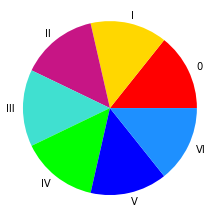
\includegraphics[width=0.4\textwidth]{rys.33.diagram.kolowy.legenda.png}
    \caption{Legenda użytych kolorów w celu oznaczenia struktur na obrazach, które należą do różnych klas. Żródło: opracowanie własne (z wykorzystaniem biblioteki \ita{matplotlib})}
    \label{rys.33.diagram.kolowy.legenda.png}
\end{figure}
Na rys \ref{rys.33.diagram.kolowy.legenda.png} została przedstawiona legenda. Każdy z siedmiu kolorów przedstawionych na wykresie kołowym odpowiada jednej z siedmiu klas strukur (zgodnie z opisem na diagramie). Kolory te zostały dobrane za pomocą generatora wizualnie odmiennych kolorów, aby były jak najbardziej wyraziste. Na poniższych obrazach (rys. \ref{rys.34} - \ref{rys.38}) 
\begin{figure}[h]
	\centering
	\begin{subfigure}{0.42\textwidth}
	    \centering
	    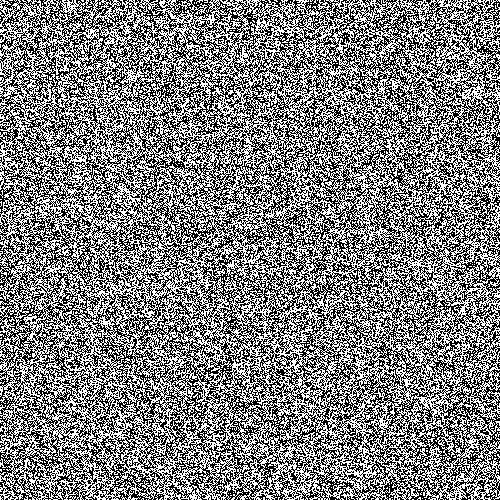
\includegraphics[width=1\textwidth]{rys.34a.pokolorowane.struktury.png}
	    \subcaption{\label{subfigure_a}Wykryte, sklasyfikowane i ubarwione struktury}
	\end{subfigure}
	\begin{subfigure}{0.42\textwidth}
	    \centering
	    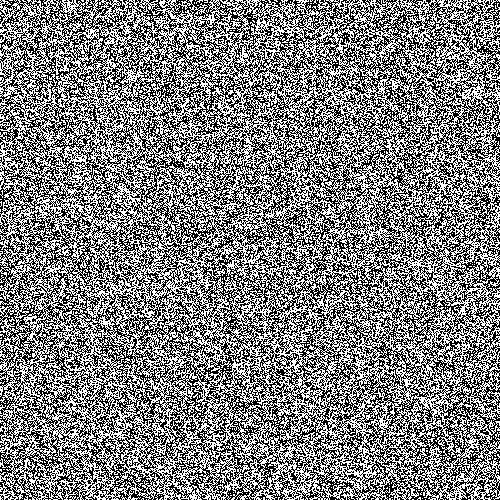
\includegraphics[width=1\textwidth]{rys.34b.oryginalne.zdjecie.png}
	    \subcaption{\label{subfigure_b}Zdjęcie mikrostruktury}
	\end{subfigure}
	\caption{\label{rys.34}Zdjęcia mikrostruktury zawierające struktury klas I-III. Źródło: opracowanie własne}
\end{figure}
obowiązuje schemat, iż po prawej stronie znajduje się oryginalne zdjęcie mikrostruktury, natomiast po lewej stronie znajduje się to samo zdjęcie, z tym że znajdujące tam struktury zostały pokolorowane zgodnie z legendą (rys. \ref{rys.33.diagram.kolowy.legenda.png}). Są to przykładowe zdjęcia, które 
\begin{figure}[h]
	\centering
	\begin{subfigure}{0.42\textwidth}
	    \centering
	    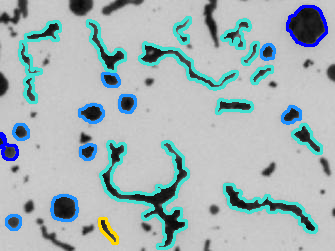
\includegraphics[width=1\textwidth]{rys.35a.pokolorowane.struktury.png}
	    \subcaption{\label{subfigure_a}Wykryte, sklasyfikowane i ubarwione struktury}
	\end{subfigure}
	\begin{subfigure}{0.42\textwidth}
	    \centering
	    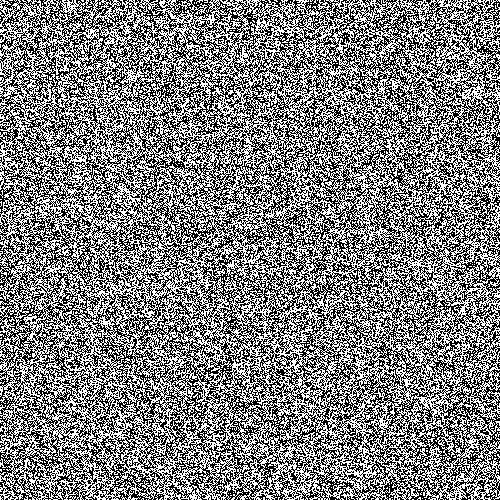
\includegraphics[width=1\textwidth]{rys.35b.oryginalne.zdjecie.png}
	    \subcaption{\label{subfigure_b}Zdjęcie mikrostruktury}
	\end{subfigure}
	\caption{\label{rys.35}Zdjęcia mikrostruktury wraz ze strukturami klasy III, V i VI. Można zauważyć również, że jedna, podłużna struktura została sklasyfikowana jako typ I. Źródło: opracowanie własne}
\end{figure}
dobrze reprezentują cały proces, który wygląda w ten sposób, że dla każdego zdjęcia wejściowego przeprowadzane są operacje opisane w rozdziale \ref{wycinanie.struktur}, a następnie są one klasyfikowane przez architekturę przedstawioną w 
\begin{figure}[h]
	\centering
	\begin{subfigure}{0.41\textwidth}
	    \centering
	    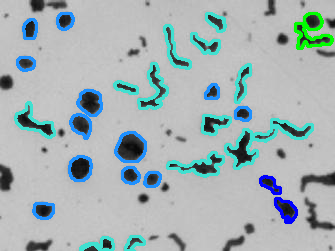
\includegraphics[width=1\textwidth]{rys.36a.pokolorowane.struktury.png}
	    \subcaption{\label{subfigure_a}Wykryte, sklasyfikowane i ubarwione struktury}
	\end{subfigure}
	\begin{subfigure}{0.41\textwidth}
	    \centering
	    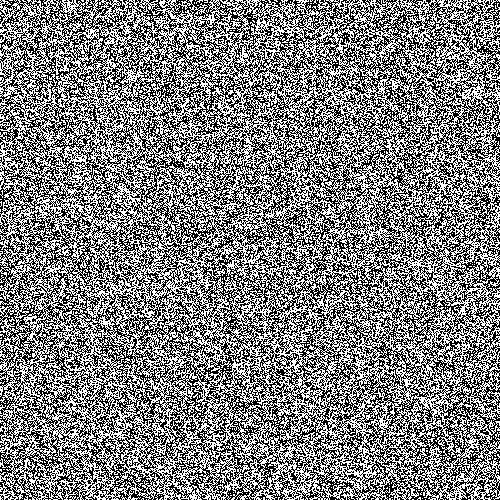
\includegraphics[width=1\textwidth]{rys.36b.oryginalne.zdjecie.png}
	    \subcaption{\label{subfigure_b}Zdjęcie mikrostruktury}
	\end{subfigure}
	\caption{\label{rys.36}Zdjęcia mikrostruktury z oznaczonymi formami grafitowymi, które należą do klas III-VI. Źródło: opracowanie własne}
\end{figure}
tym rozdziale. W związku z tym mogą wystąpić błędy, jak brak wykrycia danej struktury bądź źle sklasyfikowanie struktury.
\begin{figure}[h]
	\centering
	\begin{subfigure}{0.41\textwidth}
	    \centering
	    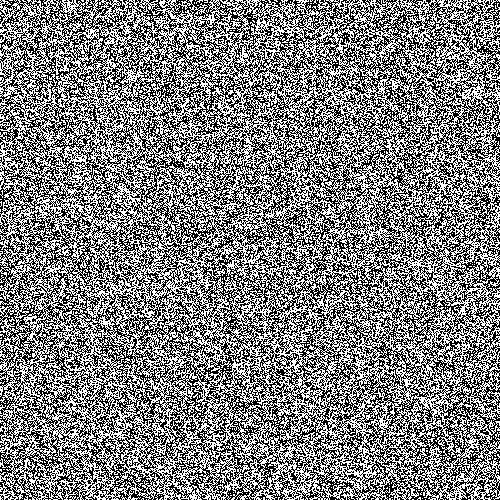
\includegraphics[width=1\textwidth]{rys.37a.pokolorowane.struktury.png}
	    \subcaption{\label{subfigure_a}Wykryte, sklasyfikowane i ubarwione struktury}
	\end{subfigure}
	\begin{subfigure}{0.41\textwidth}
	    \centering
	    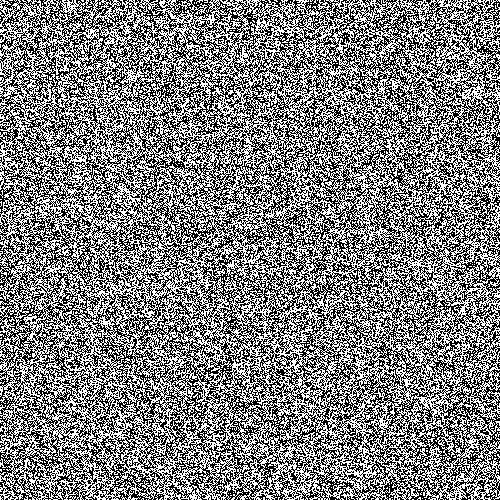
\includegraphics[width=1\textwidth]{rys.37b.oryginalne.zdjecie.png}
	    \subcaption{\label{subfigure_b}Zdjęcie mikrostruktury}
	\end{subfigure}
	\caption{\label{rys.37}Zdjęcia mikrostruktury zawierające kształty sklasyfikowane do klas IV oraz VI. Źródło: opracowanie własne}
\end{figure}
\begin{figure}[h]
	\centering
	\begin{subfigure}{0.41\textwidth}
	    \centering
	    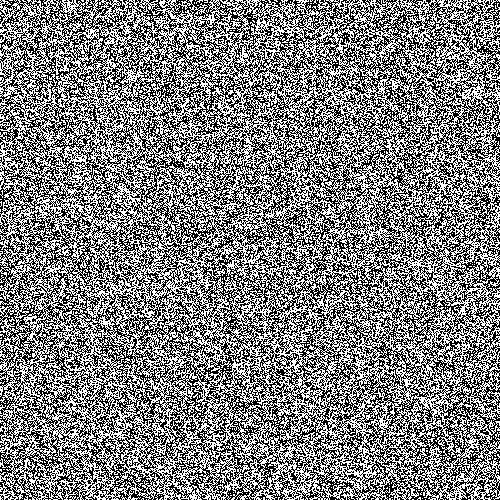
\includegraphics[width=1\textwidth]{rys.38a.pokolorowane.struktury.png}
	    \subcaption{\label{subfigure_a}Wykryte, sklasyfikowane i ubarwione struktury}
	\end{subfigure}
	\begin{subfigure}{0.41\textwidth}
	    \centering
	    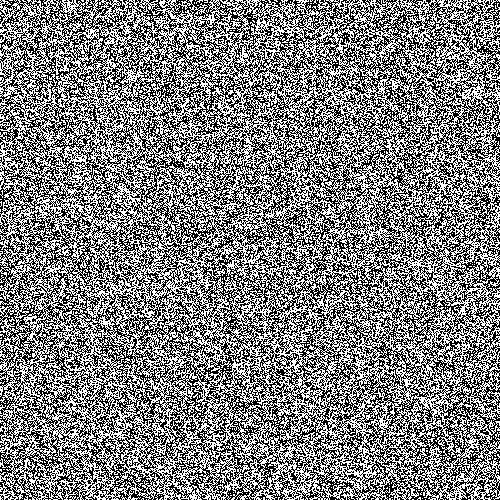
\includegraphics[width=1\textwidth]{rys.38b.oryginalne.zdjecie.png}
	    \subcaption{\label{subfigure_b}Zdjęcie mikrostruktury}
	\end{subfigure}
	\caption{\label{rys.38}Zdjęcia mikrostruktur przedstawiające kształty sklasyfikowane do klas III-VI. Źródło: opracowanie własne}
\end{figure}
%\clearpage
%\noindent 
\afterpage{\clearpage}Jak widzimy na powyższych rysunkach, sieć klasyfikująca kształty wraz z całą sekwencją rozpoznawania pojedynczych struktur przynosi całkiem przyzwoite efekty. Wizualnie nie można tutaj niczego skrytykować. Natomiast często zdarza się tak, jak już wspomniano wcześniej, że struktury te są bardzo podobne do siebie i przygotowanie ich przez specjalistę w dziedzinie metalurgii mogłoby przynieść znaczny wzrost skuteczności modelu.

Ostatnią próbą w celu poprawienia skuteczności modelu było wyeliminowanie najmniejszych struktur z klasyfikacji. Są one najbardziej problematyczne, gdyż wizualnie, praktycznie się nie różnią. Dodatkowo sam autor miał problem z przypisaniem tych struktur do konkretnej klasy. Po usunięciu tych struktur otrzymalimy skuteczność na poziomie 82\%, natomiast wartość straty logistycznej wynosi $0.8$, co jest bardzo dobrym wynikiem. Tablica pomyłek została przedstawiona na rys. \ref{rys.39.confusion.matrix.big.structures.png}. 
\begin{figure}[h]
    \centering
    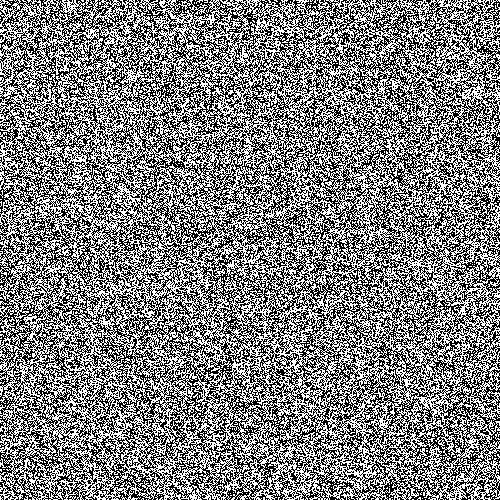
\includegraphics[width=0.7\textwidth]{rys.39.confusion.matrix.big.structures.better.quality.png}  %rys.39.confusion.matrix.big.structures.png}
    \caption{Tablica pomyłek dla klasyfikacji struktur znajdujących się na zdjęciach mikrostruktur dla danych testowych. Wykorzystano większe struktury, które zostały wybrane na podstawie zajmowanej przez nie powierzchni, jak również ich obwodu. Żródło: opracowanie własne (z użyciem biblioteki \ita{seaborn})}
    \label{rys.39.confusion.matrix.big.structures.png}
\end{figure}
Porównując te tablicę pomyłek do poprzedniej, która dotyczyła wyników badań przeprowadzonych na wszystkich danych możemy dojść do kilku ciekawych wniosków. Otóż jak pokazano w rozdz. \ref{wycinanie.struktur}, liczba struktur klasy „0"~wynosi zaledwie 14 i została dodana przez autora pracy. W tym wypadku ta klasa jest najmniej interesująca. 
Największe straty zanotowały klasy II oraz V, bo 7 i 10 punktów procentowych (odpowiednio). Natomiast największe zyski zanotowały klasy IV oraz VI, bo aż 33 i 6 punktów procentowych.

\subsection{Wnioski}
\label{klasyfikacja.struktur.wnioski}

Po badaniach nad zagaqdnieniem przedstawionym w tym rozdziale można wyciągnąć wiele interesujących wniosków:
\begin{itemize}
	\item w pierwotnym zbiorze występowały zdjęcia (przykładowo rys. \ref{fig:mesh15}), które nie nadawały się do tej analizy, gdyż nie zawierały w sobie głównych form grafitowych (rys. \ref{fig:mesh14}), aczkolwiek była to zdecydowana mniejszość,
	\item GHT zwracała dosyć precyzyjne wyniki (rys. \ref{fig:mesh23}), jednak miała wiele obostrzeń, przede wszystkim konieczność zastosowania identycznego obrazka referencyjnego do poszukiwanego, mimo to do innych zastosowań może być skutecznie wykorzystywana,
	\item gdy wykorzystano rozmycie gaussowskie (ang. \ita{Gaussian blur}), popękane struktury były wykrywane lepiej (gdyż pęknięcia nie były uznawane za struktury). Również klasy V-VI zyskiwały na skuteczności, natomiast traciły na tym pozostałe klasy (przede wszystkim I-II),
	\item przetestowano również progowanie obrazu (ang. \ita{thresholding}), które polega na binaryzowaniu zdjęć, tj. przypisywaniu im czarnych bądź białych pikseli w zależności od poprzedniej wartości tych pikseli. Miało to zapobiegać traktowaniu pęknięć jako struktury, jednakże całkowita skuteczność również spadła.
\end{itemize}

\section{Ocena jakości odlewów}
\label{Ocena jakości odlewów}

Jest to drugi najszerszy obszar badań (obok rozdz. \ref{sec:klasyfikacja_struktur}), gdyż jest to główny punkt tych badań oraz temat niniejszej pracy. Zebrano i przedstawiono tutaj wszystkie testy związane z oceną jakości odlewów. Eksperymenty przedstawiono w kolejności, w jakiej zostały wykonywane, tj. od najprostszych metod do najbardziej skomplikowanych, które jednocześnie zwracały najlepsze wyniki. Badanie rozpoczęto od sprawdzenia skuteczności klasycznych klasyfikatorów na danych w postaci momentów Hu oraz tekstur Haralicka (rozdz. \ref{sec:hu_haralick}). Następnie [TODO]

\subsection{Momenty Hu oraz tekstury Haralicka}
\label{sec:hu_haralick}

Pierwszym podejściem było wykorzystanie tekstur Haralicka i momentów Hu do zidentyfikowania struktur na zdjęciu. Implementacja metody momentów Hu została zaczerpnięta z pakietu \ita{opencv-python}, natomiast implementacja tekstur Haralicka została zaczerpnięta z modułu \ita{mahotas}. Może się wydawać, że użycie tych algorytmów jest poprawne i przyniesie pożądane rezultaty, ponieważ zostały zaprojektowane specjalnie do tego celu. Rysunek \ref{fig:mesh20} przedstawia dwa zdjęcia różnych mikrostruktur, które potencjalnie można zidentyfikować przy użyciu technik opisanych powyżej.
\begin{figure}[h]
	\centering
	\begin{subfigure}{0.47\textwidth}
	    \centering
	    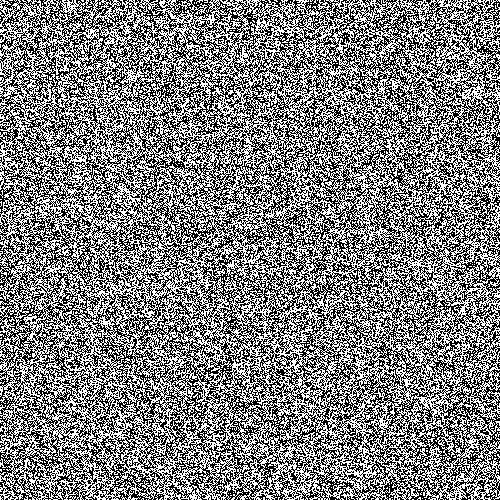
\includegraphics[width=1\textwidth]{rys.20.przyklad.mikrostruktur.a.png}
	    \subcaption{\label{subfigure_a}Zdjęcie mikrostruktury z obiektami klasy I (rys. \ref{fig:mesh14})}
	\end{subfigure}
	\begin{subfigure}{0.47\textwidth}
	    \centering
	    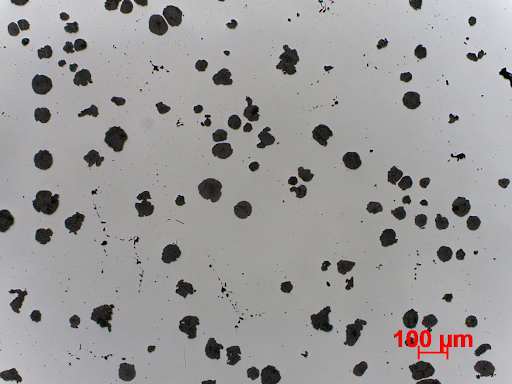
\includegraphics[width=1\textwidth]{rys.20.przyklad.mikrostruktur.b.png}
	    \subcaption{\label{subfigure_b}Zdjęcie mikrostruktury z obiektami klasy V (rys. \ref{fig:mesh14})}
	\end{subfigure}
	\caption{\label{fig:mesh20}Dwa przykładowe zdjęcia mikrostruktur. Ich tekstury i znajdujące się tam kształty diametralnie się różnią. Źródło: \cite{Pirowski17}}
\end{figure}
W pierwszym eksperymencie wykorzystano tekstury Haralicka, momenty Hu, a także modele maszyny wektorów nośnych (SVM) oraz lasów losowych (RF, RFC). 
\begin{table}[h]
	\centering
	\begin{threeparttable}
		\caption{Wyniki klasyfikacji binarnej z użyciem klasycznych klasyfikatorów, z wykorzystaniem momentów Hu oraz tekstur Haralicka. Źródło: opracowanie własne}
		\label{hu_haralick_table}
		\begin{tabularx}{1\textwidth}{ |X|X|X|X| }
		  \hline
		  \textbf{Model} & \textbf{Typ wejścia} & \textbf{Wagi klas} & \textbf{Dokładność}\\

		  \hline
		  SVM & Hu\tnote{a} & — & 71.5\%\\

		  \hline
		  SVM & Haralick\tnote{b} & — & 71.5\%\\

		  \hline
		  SVM & Hu + Haralick\tnote{c} & — & 71.5\%\\

		  \hline
		  RFC & Hu & zrównoważone & 58\%\\

		  \hline
  		  RFC & Haralick & zrównoważone & 70\%\\
  		  
		  \hline
  		  RFC & Hu + Haralick & zrównoważone & 70.1\%\\
  		  
		  \hline
		\end{tabularx}
		\begin{tablenotes}
			\footnotesize
			\item[a] Momenty Hu wyliczone ze zdjęć (7 elementów).
			\item[b] Tekstury Haralicka wyznaczone ze zdjęć (13 elementów).
			\item[c] Konkatenacja wyników dwóch powyższych metod (20 elementów).
		\end{tablenotes}
	\end{threeparttable}
\end{table}
Testy zostały przeprowadzone na zbiorze danych klasyfikowanych ze względu na wytrzymałość na rozciąganie. Niestety taka konfiguracja modeli i metod nie przyniosła oczekiwanych rezultatów. Testy przeprowadzono z wykorzystaniem sprawdzianu krzyżowego (ang. \ita{cross-validation}), a dokładnie sprawdzian \ita{k}-krotny (rozdz. \ref{cross.validation}), w którym oryginalna próba jest dzielona na \ita{k} podzbiorów, po czym każdy z tych podzbiorów jest wykorzystywany jako zbiór testowy, gdzie w tym czasie wszystkie pozostałe są wykorzystywane jako zbiór trenignowy. Następnie te \ita{k} rezultatów jest uśrednianych. 
Wyniki zaprezentowano w tabeli \ref{hu_haralick_table}.
\begin{table}[h]
	\centering
	\begin{threeparttable}
		\caption{Wyniki klasyfikacji binarnej z użyciem klasycznych klasyfikatorów, z wykorzystaniem momentów Hu oraz tekstur Haralicka. Dodatkowo rozszerzono dwukrotnie liczbę zdjęć o niskiej odporności (augmentacja). Źródło: opracowanie własne}
		\label{hu_haralick_table_with_augmentation}
		\begin{tabularx}{1\textwidth}{ |X|X|X|X| }
		  \hline
		  \textbf{Model} & \textbf{Typ wejścia} & \textbf{Wagi klas} & \textbf{Dokładność}\\

		  \hline
		  SVM & Hu & — & 55.7\%\\

		  \hline
		  SVM & Haralick & — & 54.6\%\\

		  \hline
		  SVM & Hu + Haralick & — & 54.6\%\\

		  \hline
		  RFC & Hu & zrównoważone & 56.6\%\\

		  \hline
  		  RFC & Haralick & zrównoważone & 86\%\\
  		  
		  \hline
  		  RFC & Hu + Haralick & zrównoważone & 86\%\\
  		  
		  \hline
		\end{tabularx}
	\end{threeparttable}
\end{table}
Jak widzimy, wyniki dla większości tych metod wynoszą około 71\%. Nieco gorszy wynik w przypadku lasu losowego może wynikać z zastosowania zrównoważenia wag klas. Jednakże zbiór danych składa się z 3358 zdjęć o wysokiej wytrzymałości na rozciąganie oraz 1337 zdjęć o niskiej wytrzymałości na rozciąganie (patrz \ref{sec:normalizacja_przyblizenia}). A więc liczba zdjęć o wysokiej wytrzymałości stanowi dokładnie 71\% wszystkich danych, stąd klasyfikatory zamiast rzeczywiście rozpoznawać dane tak na prawdę mogą dopasowywać się do częstotliwości występowania zdjęć określonej klasy. Stąd przeprowadzono dodatkowe testy z wykorzystaniem augmentacji (patrz \ref{cha:cha3.4}, \ref{sec:augmentacja}). Konkretnie zastosowano metodę odbicia na mniej licznej klasie (a więc na zdjęciach o niskiej wytrzymałości), dzięki czemu stosunek liczby zdjęć o wysokiej wytrzymałości do liczby wszystkich zdjęć spadł z 71\% do 55.7\%. Wyniki po przeprowadzeniu augmentacji znajdują się w tab. \ref{hu_haralick_table_with_augmentation}.
\begin{table}[h]
	\centering
	\begin{threeparttable}
		\caption{Wyniki klasyfikacji binarnej z użyciem klasycznych klasyfikatorów, z wykorzystaniem momentów Hu oraz tekstur Haralicka. Dane dodatkowo zostały zaszumione, aby zapobiec nadmiernemu dopasowaniu się modelu do danych. Źródło: opracowanie własne}
		\label{hu_haralick_table_with_augmentation_and_noise}
		\begin{tabularx}{1\textwidth}{ |X|X|X|X| }
		  \hline
		  \textbf{Model} & \textbf{Typ wejścia} & \textbf{Wagi klas} & \textbf{Dokładność}\\

		  \hline
		  SVM & Hu & — & 55.7\%\\

		  \hline
		  SVM & Haralick & — & 55.5\%\\

		  \hline
		  SVM & Hu + Haralick & — & 55.5\%\\

		  \hline
		  RFC & Hu & zrównoważone & 51.6\%\\

		  \hline
  		  RFC & Haralick & zrównoważone & 72.2\%\\
  		  
		  \hline
  		  RFC & Hu + Haralick & zrównoważone & 72.6\%\\
  		  
		  \hline
		\end{tabularx}
	\end{threeparttable}
\end{table}
Dodatkowo, aby nie zwiększać sztucznie dokładności ze względu na podobieństwo danych wygenerowanych sztucznie i oryginalnych, postanowiono nałożyć szum na dane wygenerowane syntetycznie. Zdecydowano się na szum biały. Wyniki zostały przedstawione w tabeli \ref{hu_haralick_table_with_augmentation_and_noise}.

Porównując wyniki otrzymane w tych trzech eksperymentach można dojść z penwością do kilku wniosków. Po pierwsze, widać wyraźnie, że wyniki pomiędzy modelami drzew oraz maszyny wektorów znacząco się różnią. W pierwszym eksperymencie wyniki dla SVM są lepsze od 1 do nawet 12 punktów procentowych. W pozostałych dwóch eksperymentach wyniki dla SVM są znacznie gorsze od tych dla lasu losowego, w ekstremalnym przypadku aż o 30 punktów procentowych. Po drugie, można zauważyć, że w większości przypadków wyniki dla momentów Hu są najgorsze, co można wytłumaczyć tym, iż jest to najprostsza metoda. Natomiast widzimy również wpływ augmentacji danych, jak również zaszumienia danych. Można przyjąć, iż najbardziej wiarygodne wyniki otrzymaliśmy w trzecim eksperymencie, gdyż, przede wszystkim, skuteczność algorytmu nie pokrywa się ze stosunkiem liczebności klas, oraz wyniki nie różnią się między sobą w niewytłumaczalny sposób. Mimo wszystko, ciężko do końca ocenić co tak naprawdę wpłynęło na te wyniki. Dodatkowo to podejście ma bardzo niską interpretowalność, tzn. ciężko ocenić dlaczego model wybrał jedną decyzję, zamiast innej. Natomiast atutem tego podejścia jest czas wykonywania (czas uczenia modeli). Mimo ustawienia parametrów SVM na wiele iteracji, a także ustawienie stosunkowo dużej liczby drzew dla algorytmu lasu losowego, czas uczenia tych modeli jest rzędu kilkunastu sekund. Jak widzimy, już nawet najprostsze metody dają pewne pozytywne rezultaty, dlatego zdecydowano się na nieco bardziej złożoną strategię, która być może podniesie skuteczność.

\subsection{Klasyfikacja wytrzymałości na rozciąganie za pomocą liczby struktur na obrazach}
\label{Klasyfikacja za pomocą liczby struktur}

W następnym kroku przetestowano skuteczność klasycznych klasyfikatorów w ocenie jakości odlewów (tj. predykcji wytrzymałości na rozciąganie odlewów). Jako dane wejściowe zastosowano liczbę struktur poszczególnych klas (rys. \ref{fig:mesh14}), które są pozyskiwane w procesoe przedstawionym w rozdz. \ref{sec:klasyfikacja_struktur}. Stąd na wejście klasycznych klasyfikatorów jest podawana tablica siedmiu liczb, z czego każda z tych liczb odpowiada liczebności odpowiedniej klasy (tj. liczba „zerowa"~odpowiada liczebności obiektów klasy „0"~itd.) i na podstawie tych danych starają się przewidzieć wytrzymałość na rozciąganie odlewów przedstawianych na zdjęciach, których te dane dotyczą. 
\begin{figure}[h]
    \centering
    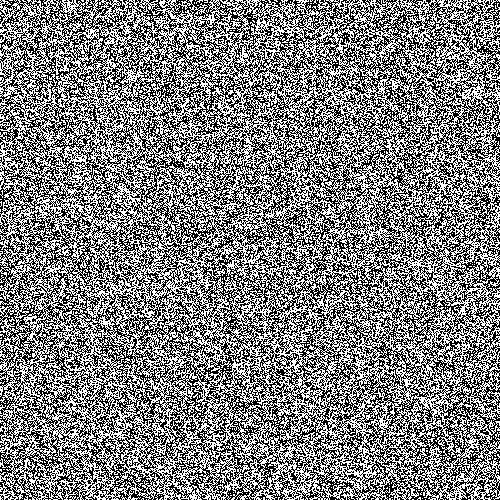
\includegraphics[width=0.75\textwidth]{rys.41.flowchart.diagram.png}
    \caption{Schemat blokowy przedstawiający działanie klasyfikacji wytrzymałości na rozciąganie na podstawie liczności struktur poszczególnych klas. Żródło: opracowanie własne (z wykorzystaniem \href{https://www.lucidchart.com}{lucidchart})}
    \label{rys.41.flowchart.diagram.png}
\end{figure}
Przetestowano również podejścia, w których zamiast bezwzględnych liczb podawano na wejście procentowy udział struktur poszczególnych klas, a także strategie, w której na wejście podawano wynik funkcji softmax (wzór \ref{eq.softmax}) na bezwzględnych licznościach struktur poszczególnych klas. Na rys. \ref{rys.41.flowchart.diagram.png} przedstawiono schemat działania całego procesu.
W tym celu wykorzystano najpopularniejsze klasyfikatory, jak maszyna wektorów nonych (SVM), drzewo decyzyjne (DT, rozdz. \ref{cha:Drzewo decyzyjne}), las losowy (RFC, rozdz.\ref{cha:Las losowy}), regresja logistyczna (rozdz. \ref{Regresja logistyczna}), perceptron wielowarstwowy (MLP, rozdz. \ref{cha:Siecineuronowe}) oraz AdaBoost (rozdz. \ref{AdaBoost}). W następnych podrozdziałach są przedstawione analizy oraz wyniki uzyskane z użyciem wyżej wymienionych klasyfikatorów.

\subsubsection{Klasyfikator SVM}
\label{structures.with.svm}

Jako pierwsze zostanie omówione podejście, w którym jako klasycznego klasyfikatora użyto SVM, czyli maszynę wektorów nośnych (rozdz. \ref{cha:Maszyna wektorów nośnych}). Schemat ogólny został przedsawiony na rys. \ref{rys.41.flowchart.diagram.png}. W pierwszej kolejności przebadano strategię, w której na wejście SVM podawano bezwzględną liczbę struktur poszczególnych klas. Badania przeprowadzono wykorzystując walidację krzyżową (rozdz. \ref{cross.validation}) oraz przeszukiwanie siatki (rozdz. \ref{Optymalizacja hiperparametrów}). Użyto już gotowej implementacji z biblioteki \ita{scikit-learn} pod nazwą \ita{GridSearchCV}, który obsługuje te dwie rzeczy naraz. W rezultacie otrzymano model, który osiągnął 82.7\% dokładności dla danych testowych oraz cztery punkty procentowe więcej dla danych treningowych. Wartość straty logistycznej wyniosła $5.96$. To oznacza, że nie doszło do przetrenowania, ani niedotrenowania modelu do danych, czemu też zapobiega sprawdzian krzyżowy. W każdym razie wyniki wydają się być wysokie, tym bardziej, że opierają się na modelu, który miał mniejszą skuteczność (o pół punktu procentowego). Poniżej przedstawiono wykres krzywej Precision-Recall, który wskazuje jaka jest precyzja modelu (ang. \ita{precision}) przy zadanej czułości (ang. \ita{recall}). 
\begin{figure}[h]
    \centering
    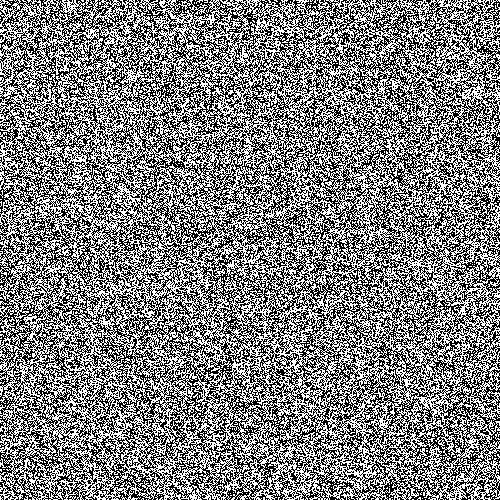
\includegraphics[width=0.62\textwidth]{rys.42.krzywa.precision.recall.png}
    \caption{Wykres krzywej Precision-Recall. Średnia wartość precyzji wynosi 0.88. Żródło: opracowanie własne (z wykorzystaniem biblioteki \ita{scikit-learn})}
    \label{rys.42.krzywa.precision.recall.png}
\end{figure}
Natomiast na rys. \ref{rys.43.confusion.matrix.svm.unbalanced} przedstawiono tablicę pomyłek dla tej klasyfikacji.
\begin{figure}[h]
    \centering
    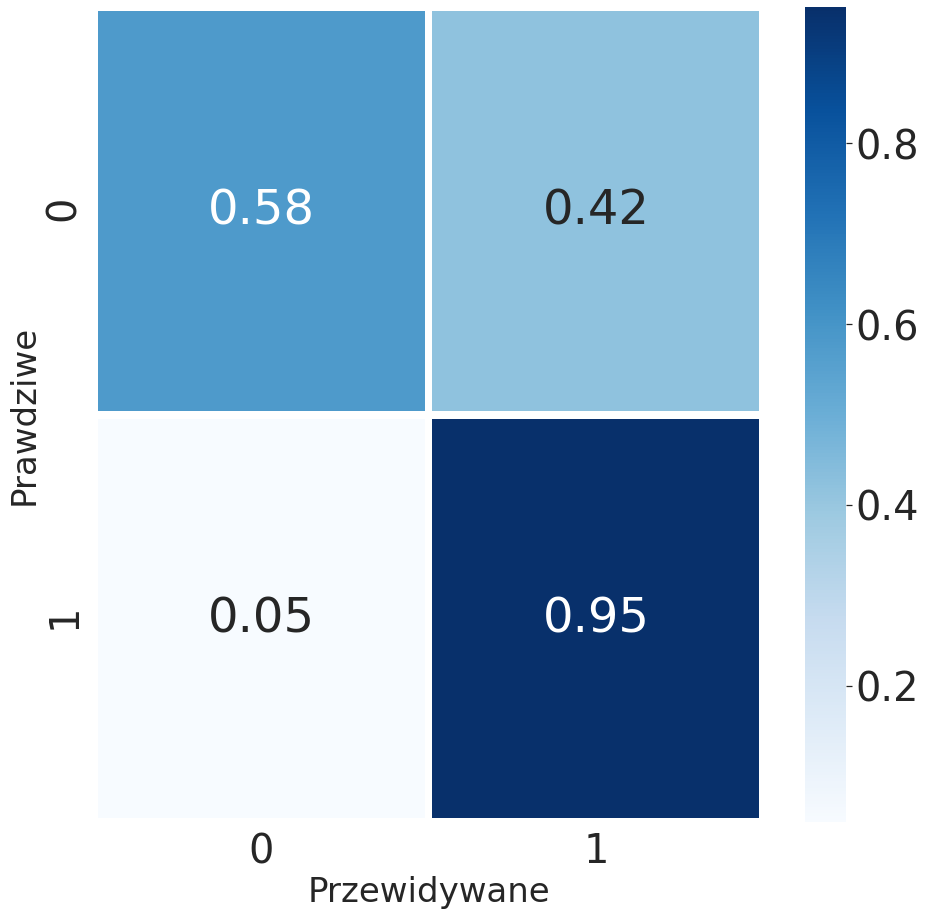
\includegraphics[width=0.45\textwidth]{rys.43.confusion.matrix.svm.unbalanced}
    \caption{Tablica pomyłek dla klasyfikacji wytrzymałości na rozciąganie odlewów. Użyto niezbalansowanych danych (oryginalny zbiór). Żródło: opracowanie własne (z wykorzystaniem biblioteki \ita{seaborn})}
    \label{rys.43.confusion.matrix.svm.unbalanced}
\end{figure}

Kolejnym przetestowanym pomysłem była strategia, w której zamiast bezwzględnych liczb okrelających liczność struktur odpowiednich klas na wejście podawano procentowy udział struktur poszczególnych klas. Tym razem skuteczność wyniosła $78.7\%$, a więc dokładnie o cztery punkty procentowe mniej, niż w przypadku liczności struktur. Średnia wartość precyzji wyniosła $0.8$, a więc również gorzej niż w poprzednim wypadku. Również wartość straty logistycznej jest większa i wynosi $7.37$. Stąd wykres nie jest nawet wymagany, ponieważ po samych wynikach liczbowych możemy z całą pewnością stwierdzić, iż tutaj lepiej zadziałało poprzednie podejście. Próbując wyjaśnić takie rozbieżności tak naprawdę ciężko dojść do sensownego wyjaśnienia tej sytuacji. Wydawać mogłoby się, iż wyniki powinny być znacznie bardziej zbliżone, a to ze względu na charakter danych wejściowych. Procentowy udział struktur poszczególnych to nic innego jak znormalizowane wyniki biorące pod uwagę liczność struktur danej klasy względem wszystkich pozostałych. A jednak wyniki są dużo gorsze. Natomiast wystąpiła jedna drobna różnica, a mianowicie było dziewięć zdjęć, dla których nie wykryto ani jednej struktury, stąd niemożliwe było wyliczenie względnego udziału struktur poszczególnych klas, wskutek czego konieczne było ich wyeliminowanie ze zbioru. Tak czy inaczej, jest to tylko dziewięć przykładów spośród 4695 wszystkich, stąd można ten fakt pominąć. 

Jako ostatnia została przetestowana strategia, w której na wejście klasycznych klasyfikatorów jest podawany wynik funkcji softmax na pierwotnych danych (tj. liczności struktur poszczególnych klas). W tym przypadku otrzymaliśmy dokładność na poziomie $79\%$, średnią wartość precyzji równą $0.72$ oraz wartość straty logistycznej równą $7.21$. Jak widzimy, z wszystkich trzech zasosowanych tutaj strategii najlepiej sprawdza się bezwzględna liczność struktur poszczególnych klas, dlatego w dalszych badaniach będziemy się głównie skupiać na tego typu danych. 

Jednakże dane są mocno niezbalansowane, co zostało pokazane w rozdz. \ref{sec:normalizacja_przyblizenia}. W ramach przypomnienia, zdjęć reprezentujących odlewy z wysoką wytrzymałością na rozciąganie jest 3358, natomiast tych z niską jest 1337. To mogłoby wyjaśniać przesunięcie w stronę klasy odpowiadającej wysokiej wytrzymałości, co zostało przedstawione na rys. \ref{rys.43.confusion.matrix.svm.unbalanced} (tzw. błąd drugiego rodzaju). Co prawda zgodnie z terminologią jest to zaledwie „delikatnie niezbalansowany zbiór", aczkolwiek warto sprawdzić czy to niezrównoważenie ma wpływ na wyniki.
\begin{figure}[h]
    \centering
    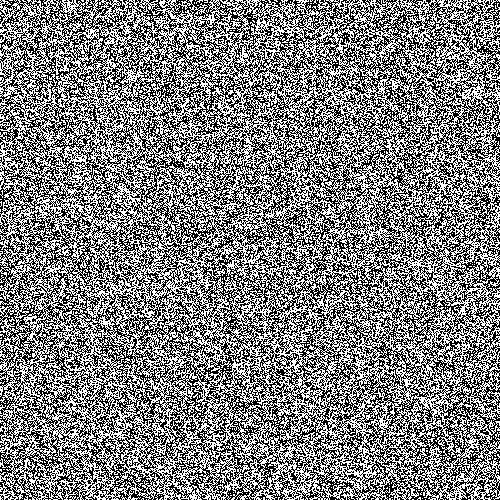
\includegraphics[width=0.45\textwidth]{rys.44.confusion.matrix.svm.balanced}
    \caption{Tablica pomyłek dla klasyfikacji wytrzymałości na rozciąganie odlewów. Dane zostały zbalansowane. Źródło: opracowanie własne (z wykorzystaniem biblioteki \ita{seaborn})}
    \label{rys.44.confusion.matrix.svm.balanced}
\end{figure}
W tym celu wykorzystano najprostszą technikę równoważenia zbiorów, a mianowicie wyeliminowano z danych nadmiarowe przykłady nadreprezentowanej klasy. W ten sposób mamy teraz 1337 przykładów zarówno mikrostruktur wysokiej, jak i niskiej wytrzymałości. Jednakże po zbalansowaniu klas problem nadal występuje (rys. \ref{rys.44.confusion.matrix.svm.balanced}). Przeprowadzono te same testy i wartości wszystkich metryk się pogorszyły, mimo że tablica pomyłek po tym zabiegu wygląda nieco lepiej. Stąd wiadomo, że przesunięcie w stronę klasy wysokich wytrzymałości nie jest kwestią niezbalansowania klas. Co jest przyczyną tego stanu rzeczy postaramy się dogłębniej wyjaśnić przy okazji testów kolejnych klasyfikatorów klasycznych, w tym bardziej interpretowalnych (m.in. drzewa decyzyjne) w kolejnych podrozdziałach.

Podsumowując wyniki badań dla SVM przygotowano szkic, w którym są przedstawione zbiorczo zebrane wyniki (tab. \ref{svm.binary.summary.table}). 
\begin{table}[h]
	\centering
	\begin{threeparttable}
		\caption{Podsumowanie wyników klasyfikacji binarnej z użyciem klasyfikatora SVM w celu predykcji wytrzymałości na rozciąganie odlewów}
		\label{svm.binary.summary.table}
		\begin{tabularx}{1\textwidth}{ |X|X|X|X| }
		  \hline
		  \textbf{Typ wejścia} & \textbf{Dokładność} & \textbf{AP\tnote{a}} & \textbf{Strata logistyczna}\\

		  \hline
		  Liczba struktur & \bo{82.7\%} & \bo{0.88} & \bo{5.96}\\

		  \hline
		  Procentowy udział struktur & 78.7\% & 0.8 & 7.37\\

		  \hline
		  Wartość funkcji softmax dla liczby struktur & 79\% & 0.72 & 7.21\\

		  \hline
		  Liczba struktur (zbalansowane dane)  & 78.4\% & 0.79 & 7.35\\
%
%		  \hline
%  		  Optuna i kroswalidacja & \bo{84\%} & \bo{0.88} & \bo{5.66}\\
%  		  
		  \hline
		\end{tabularx}
		\begin{tablenotes}
			\footnotesize
			\item[a] AP – średnia wartość precyzji.
		\end{tablenotes}
	\end{threeparttable}
\end{table}
Widzimy, że najlepsze wyniki otrzymujemy dla oryginalnych danych wejściowych, tj. w postaci liczności struktur poszczególnych klas, stąd w kolejnych badaniach z użyciem pozostałych klasyfikatorów skupimy się głównie na tego typu danych.
Dodatkowo, w ramach próby uzyskania najlepszego możliwego wyniku skorzystano z biblioteki \ita{Optuna}, która służy do optymalizacji hiperparametrów. Polega ona na nieco innym wyszukiwaniu, niż w przypadku poprzedniego modułu. Po zastosowaniu kroswalidacji ta strategia przyniosła najlepsze wyniki. Dla danych w postaci liczby struktur otrzymujemy $84\%$ dokładności, $0.88$ średniej wartości precyzji oraz $5.66$ wartości straty logistycznej.

%%%%%%%%% DRZEWO DECYZYJNE %%%%%%%%%%
\subsubsection{Drzewo decyzyjne}
\label{structures.with.dt}

W tym podrozdziale zajmiemy się wynikami osiąganymi za pomocą drzew decyzyjnych (\ref{cha:Drzewo decyzyjne}). Mimo, iż jest to bardzo prosty model, często zwraca przyzwoite wyniki, zaś jego interpretowalność jest jego największym atutem (obok jego prostoty). 
Jak wiemy istnieje wiele algorytmów generowania drzew decyzyjnych. Jako że autor czerpie implementacje klasycznych klasyfikatorów z biblioteki \ita{scikit-learn}, toteż pierwszym przebadanym algorytmem będzie ten wykorzystywany przez wspomnianą bibliotekę. Jest to zoptymalizowana wersja algorytmu CART.
Ponownie rozpoczniemy od zaprezentowania wyników, gdy jako dane wejściowe wykorzystano bezwzględną liczność struktur poszczególnych klas. Testy podzielono względem głębokości testowanych drzew. Ponieważ wymiar danych wejściowych wynosi siedem, nie ma sensu bliżej przyglądać się drzewom o głębokości większej niż trzy. Natomiast w ramach porównania również one zostaną uwzględnione w podsumowaniu. 
\begin{figure}[h]
    \centering
    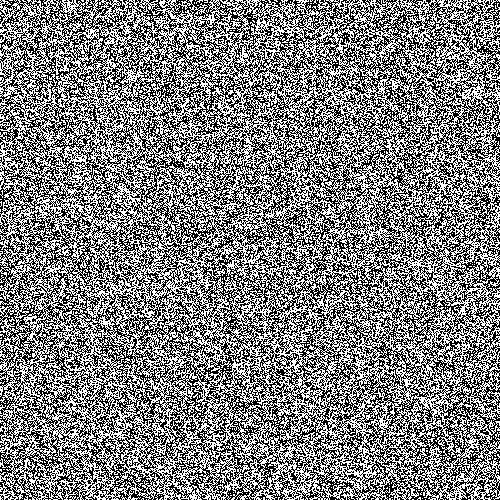
\includegraphics[width=0.5\textwidth]{rys.45.decision.tree.depth.1}
    \caption{Wizualizacja drzewa decyzyjnego. Warunek jest przedstawiony w pierwszym wierszu pierwszego klocka decyzyjnego. Sprawdzamy, czy struktur III typu jest mniej lub równo $2.5$. Na tej podstawie jest wyznaczana wytrzymałość odlewu. Źródło: opracowanie własne (z wykorzystaniem biblioteki \ita{graphviz})}
    \label{rys.45.decision.tree.depth.1}
\end{figure}
W pierwszej kolejności przeprowadzono badania dla drzew o głębokości równej jeden. Dla takich drzew średnia dokładność modelu wynosi 78\%, co już jest bardzo dobrym wynikiem. Wizualizacja takiego drzewa została przedstawiona na rys. \ref{rys.45.decision.tree.depth.1}. 
Jak możemy zauważyć, najważniejsze są tutaj struktury typu III (rys. \ref{fig:mesh14}). Biorąc pod uwagę tylko ten jeden typ struktur otrzymujemy dokładność na wspomnianym poziomie 78\%. Zobaczmy teraz jak prezentują się wyniki dla drzewa o głębokości równej dwa. Otóż dokładność wyniosła 81.2\%, natomiast wizualizacja została przedstawiona na rys. \ref{rys.46.decision.tree.depth.2}. 
\begin{figure}[h]
    \centering
    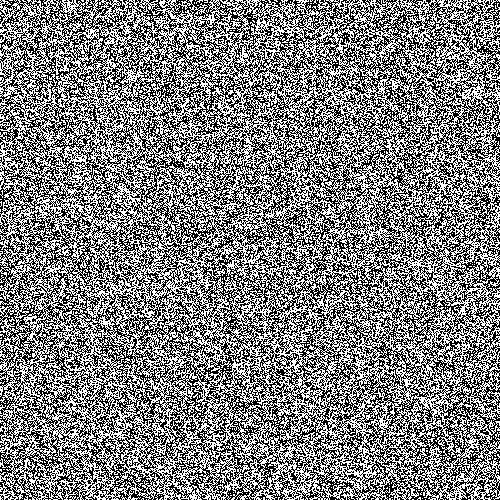
\includegraphics[width=0.85\textwidth]{rys.46.decision.tree.depth.2}
    \caption{Wizualizacja drzewa decyzyjnego o głębokości równej dwa. Źródło: opracowanie własne (z wykorzystaniem bibliteki \ita{graphviz})}
    \label{rys.46.decision.tree.depth.2}
\end{figure}
Jak możemy zauważyć, klasa III jest ponownie najważniejszą klasą, natomiast dochodzą nam również klasy I oraz VI. Logicznym wytłumaczeniem tego stanu rzeczy może być fakt, iż właśnie struktury tych trzech klas najbardziej różnią się od pozostałych wizualnie. Dla drzewa o głębokości równej trzy otrzymujemy dokładność na poziomie 81.3\%, a więc zaledwie jedną dziesiątą punktu procentowego więcej, niż dla drzewa o głębokości dwa. To może świadczyć o nadmiernym dopasowaniu się modelu do danych, czy też słabej generalizacji. Dla większych głębokości drzewa nie odnotowano wzrostu dokładności. Ciekawie również prezentują się wyniki dla innych typów wejść, toteż zostaną one przedstawione na samym końcu tej sekcji w formie tabeli. 

Tymczasem przejdziemy do kolejnego algorytmu generowania drzewa decyzyjnego. Obok algorytmu CART przetestowano również algorytm ID3, którego implementacja została zaczerpnięta z biblioteki \ita{decision-tree-id3}. 
\begin{figure}[h]
    \centering
    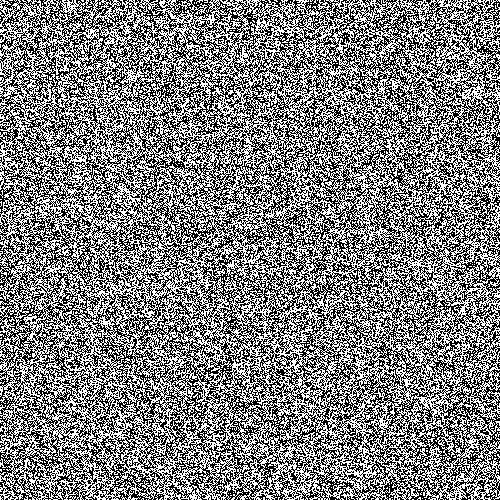
\includegraphics[width=0.55\textwidth]{rys.47.cart.vs.id3.czas.uczenia}
    \caption{Wykres przedstawiający czas uczenia modeli za skonstruowanych przy pomocy różnych algorytmów generowania drzewa, w zależności od jego głębokości. Źródło: opracowanie własne (z wykorzystaniem biblioteki \ita{matplotlib})}
    \label{rys.47.cart.vs.id3.czas.uczenia}
\end{figure}
Skonfrontowano ze sobą takie cechy, jak czas uczenia, czas zwracania wyników czy też dokładność. W pierwszej kolejności przyjrzymy się czasom uczenia tych modeli w zależności od wykorzystanego alogrytmu oraz głębokości drzew. Na rys. \ref{rys.47.cart.vs.id3.czas.uczenia} przedstawiono wyniki tego porównania.
Jak możemy zauważyć, czas uczenia jest wyraźnie dłuższy dla algorytmu ID3 i rośnie wraz ze wzrostem głębokości drzewa. Jest to znana własność tych algorytmów, gdyż na ogół algorytm CART działa szybciej, szczególnie gdy korzystamy z zoptymalizowanej wersji algorytmu CART. 

Następną metryką jest czas uzyskania wyniku. Wyniki tego porównania przedstawiono na rys. \ref{rys.48.cart.vs.id3.czas.wyniku}. 
\begin{figure}[h]
    \centering
    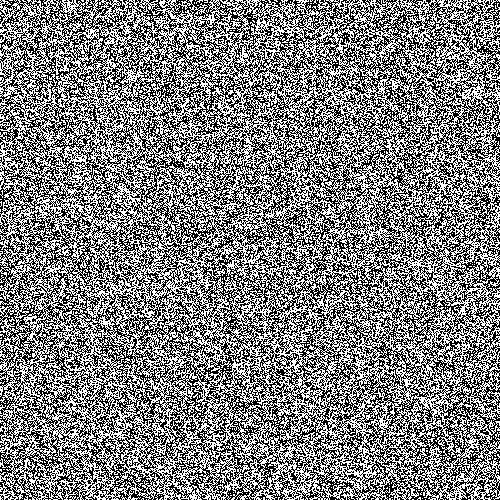
\includegraphics[width=0.5\textwidth]{rys.48.cart.vs.id3.czas.wyniku}
    \caption{Wykres przedstawiający czas uzyskania wyniku przez modele skonstruowane przy pomocy różnych algorytmów generowania drzewa, w zależności od jego głębokości. Źródło: opracowanie własne (z wykorzystaniem biblioteki \ita{matplotlib})}
    \label{rys.48.cart.vs.id3.czas.wyniku}
\end{figure}
Jak możemy zauważyć na wykresie, również w tym zestawieniu lepiej prezentuje się algorytm CART. Jego wyjście jest zwracane niemal natychmiast, natomiast na wyniki drzewa zbudowanego za pomocą algorytmu ID3 trzeba czekać dłużej i czas ten wydłuża się jeszcze bardziej, gdy obsługujemy głębsze drzewa. 

Ostatnią metryką, która posłuży nam do porównania tych dwóch algorytmów będzie dokładność. 
\begin{figure}[h]
    \centering
    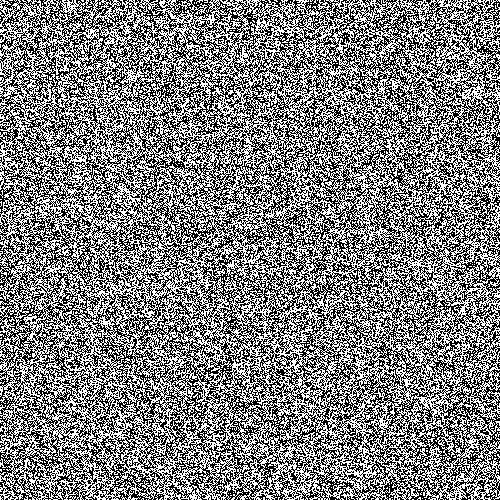
\includegraphics[width=0.5\textwidth]{rys.49.cart.vs.id3.dokladnosc}
    \caption{Wykres przedstawiający dokładność uzyskaną przez modele skonstruowane przy pomocy różnych algorytmów generowania drzewa, w zależności od jego głębokości. Źródło: opracowanie własne (z wykorzystaniem biblioteki \ita{matplotlib})}
    \label{rys.49.cart.vs.id3.dokladnosc}
\end{figure}
Otóz postaramy się zbadać który algorytm generuje bardziej dokładne drzewa pod względem klasyfikacji. 
Jak wiadomo, różne algorytmy generowania drzewa stosują różne kryteria podziału drzewa. I tak algorytm ID3 wykorzystuje entropię (ang. \ita{entropy}) lub też przyrost informacji (ang. \ita{information gain}). Z drugiej strony algorytm CART może korzystać przykładowo z miary nieczystości Giniego (ang. \ita{Gini impurity}). Stąd mogą wynikać rozbieżności w dokładności tych drzew. Na rys. \ref{rys.49.cart.vs.id3.dokladnosc} przedstawiono porównanie tych wyników. 
Widzimy, że orientacyjnie wyniki są bardzo zbliżone. Nie można jednoznacznie stwierdzić które z tych podejść jest dokładniejsze, gdyż w zależności od głębokości raz jeden, raz drugi model osiąga nieznacznie lepsze wyniki. Jednakże biorąc pod uwagę poprzednie czynniki wydaje się, że algorytm CART może być faktycznie lepszym wyborem, głównie, jeli trenujemy głębokie drzewo i zależy nam na czasie, uwzględniając w tym czas uzyskania wyników.

Na koniec, zanim przedstawimy tabelę podsumowująca wszystkie testy związane z drzewem decyzyjnym, przyjrzymy się jeszcze wynikom osiąganym za pomocą drzewa decyzyjnego skonstruowanego przy pomocy algorytmu CART, gdy uprzednio zbalansujemy dane. 
Rys. \ref{rys.50.decision.tree.depth2.balanced} przedstawia wizualizację drzewa skonstruowanego za pomocą algorytmu CART używając optymalizacji hiperparametrów. Dokładność tego modelu wynosi $73.5\%$, a więc zanotowaliśmy spadek o $7.7$ punktu procentowego. 
\begin{figure}[h]
    \centering
    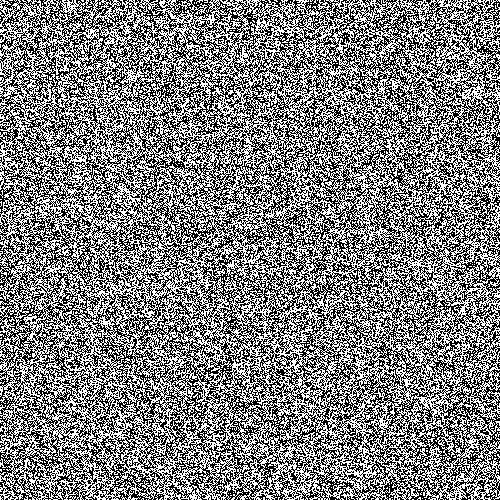
\includegraphics[width=0.85\textwidth]{rys.50.decision.tree.depth2.balanced}
    \caption{Wizualizacja drzewa decyzyjnego o głębokości równej dwa. Dodatkowo zbalansowano dane oraz użyto optymalizacji hiperparametrów. Źródło: opracowanie własne (z wykorzystaniem biblioteki \ita{graphviz})}
    \label{rys.50.decision.tree.depth2.balanced}
\end{figure}
Możemy zauważyć, iż liczność struktury typu III jest tu decydująca. Gdy jest tych struktur pewna ilość (więcej niż dwie), to wtedy z dużą pewnością możemy stwierdzić, iż struktura ma małą wytrzymałość na rozciąganie. W przeciwnym przypadku (a więc gdy struktur jest mniej niż trzy) klasyfikacja nie jest już taka dokładna. Stąd można wyciągnąć wnioski, iż obecność struktur typu III powoduje, że struktura ma niską wytrzymałość na rozciąganie.
\begin{figure}[h]
    \centering
    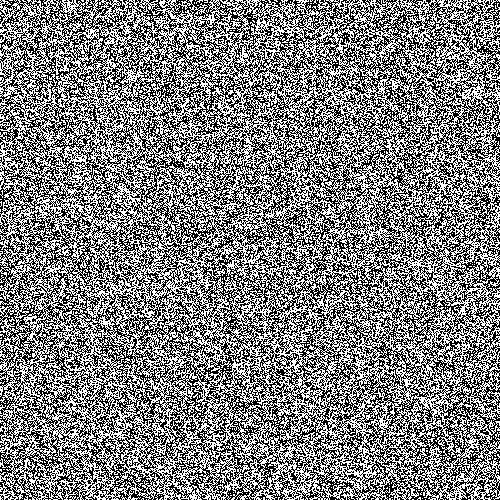
\includegraphics[width=0.5\textwidth]{rys.51.confusion.matrix.dt.balanced}
    \caption{Tablica pomyłek dla klasyfikacji wytrzymałości na rozciąganie odlewów wykorzystując drzewo decyzyjne o głębokości równej dwa. Testy przeprowadzono na zbalansowanych danych. Źródło: opracowanie własne (z wykorzystaniem biblioteki \ita{seaborn})}
    \label{rys.51.confusion.matrix.dt.balanced}
\end{figure}
Tablica pomyłek została przedstawiona na rys. \ref{rys.51.confusion.matrix.dt.balanced}. Jak można zauważyć, klasyfikacja jest nieco przesunięta w stronę wysokiej wytrzymałości (klasa 1). Można to wytłumaczyć przy pomocy wizualizacji drzewa (rys. \ref{rys.50.decision.tree.depth2.balanced}). Gdy struktur typu III jest mniej niż trzy, dokładność naszej klasyfikacji wynosi około $69\%$ (lewe poddrzewo). A ponieważ większość obecnych tam struktur ma wysoką wytrzymałość, stąd przesunięcie w kierunku tej klasy. Natomiast widzimy również spadki skuteczności w wykrywaniu wysokiej wytrzymałości, co nastąpiło wskutek ograniczenia liczby danych o tej własności. O ile wyniki są teraz bardziej wiarygodne, o tyle widzimy, że za pomocą samych liczności struktur nie jestemy w stanie stwierdzić z bardzo wysoką skutecznością jaka jest wytrzymałość tej struktury. Stąd teza, iż sieci neuronowe oceniające tę cechę odlewów na podstawie pikseli mogą osiągać wyższe skuteczności wydaje się jeszcze bardziej prawdopodobna. 

Jako podsumowanie prac z drzewami decyzyjnymi zostaje przedstawiony szkic (tab. \ref{dt.binary.summary.table}), który zawiera wyniki większości wartych uwagi testów, również tych, które nie zostały tutaj bliżej opisane.
\begin{table}[h]
	\centering
	\begin{threeparttable}
		\caption{Podsumowanie wyników klasyfikacji binarnej z użyciem drzew decyzyjnych w celu predykcji wytrzymałości na rozciąganie odlewów}
		\label{dt.binary.summary.table}
		\begin{tabularx}{1\textwidth}{ |X|X|X|X|X| }
		  \hline
		  \textbf{Typ wejścia} & \textbf{Głębokość} & \textbf{Dane zbalansowane} & \textbf{Dokładność}\\

		  \hline
		  Liczność\tnote{a} & 1 & Nie  & 78\%\\

		  \hline
		   Liczność & 2 & Nie & 81.2\%\\

		  \hline
  		  Liczność & 2 & Tak & 73.5\%\\

		  \hline
		  Liczność & 3 & Nie & 81.4\%\\

		  \hline
		  Liczność & Brak limitu & Nie & \bo{84.3\%} \\

%		  \hline
		\Xhline{3\arrayrulewidth}
  		  Procent\tnote{b} & 1 & Nie & 75\%\\
  		  
		  \hline
  		  Procent & 2 & Nie & 79\%\\
  		  
		  \hline
  		  Procent & 3 & Nie   & \bo{80\%} \\

%		  \hline
          	\Xhline{3\arrayrulewidth}
  		  Softmax\tnote{c} & 1 & Nie   & 74.5\%\\

		  \hline
  		  Softmax & 2 & Nie   & 75\% \\

		  \hline
  		  Softmax & 3 & Nie   & \bo{78\%} \\

		  \hline
		\end{tabularx}
		\begin{tablenotes}
			\footnotesize
			\item[a] Liczność struktur poszczególnych klas.
			\item[b] Procentowy udział struktur poszczególnych klas.
			\item[c] Wartość funkcji softmax dla liczności struktur.
		\end{tablenotes}
	\end{threeparttable}
\end{table}
Oczywiście najlepsze wyniki otrzymujemy dla głębszych drzew. Jednakże warto zauważyć przede wszystkim, na dwie rzeczy. Po pierwsze, po zbalansowaniu danych zanotowaliśmy znaczny spadek skuteczności, co już zostałe omówione wyżej w tym podrozdziale. Po drugie, najwyższą dokładność uzyskujemy dla danych w postaci bezwzględnej liczności struktur poszczególnych klas, nieco gorsze wyniki, gdy na wejściu podajemy procentowy udział struktur poszczególnych klas, a najgorsze wyniki, gdy użyjemy funkcji softmax. Poniekąd jest zrozumiałe, że dla funkcji softmax otrzymujemy nieco gorsze wyniki, gdyż usuwa ona z danych pewną informację. Natomiast spadek dla danych w postaci procentowego udziału jest nietypowy, aczkolwiek podobne wyniki uzyskano dla modelu SVM. Proste wytłumaczenie może opierać się na tym, iż tak na prawdę większy wpływ na wytrzymałość struktur ma to, czy struktury konkretnej klasy w ogóle wystąpiły niż stosunek ich liczności względem pozostałych klas.

\subsubsection{Las losowy}
\label{structures.with.rfc}

[bla bla] kolejne do testowania są lasy losowe.

% chyba bym się w sumie nie trzymał tego schematu, tylko chronologicznie i jednoczesnie Rm i Rp ;d
%5.2. Opis wykonanych badań i testów oraz własnej implementacji
%
%5.3. Omówienie wyników uzyskanych za pomocą metod klasycznych
%
%5.3.1. Analiza wytrzymałości na rozciąganie
%
%5.3.2. Analiza granicy plastyczności
%
%5.4. Omówienie wyników uzyskanych za pomocą sieci neuronowych
%
%5.4.1. Analiza wytrzymałości na rozciąganie
%
%5.4.2. Analiza granicy plastyczności
%
%5.5. Omówienie wyników / całościowe

